\documentclass[10pt,openany]{article}
\usepackage{ctex} 
\usepackage{geometry,graphicx,xcolor,color}
\geometry{
	a4paper,
	top=25.4mm, bottom=25.4mm,
	left=20mm, right=20mm,
	headheight=2.17cm,
	headsep=4mm,
	footskip=12mm
}
\usepackage{amssymb,amsmath,mathrsfs}             
\usepackage{mathpazo}
\usepackage[nofontspec]{newpxtext}
\usepackage{array}
\usepackage{amsmath}
\usepackage{amssymb}
\usepackage{enumerate}
\usepackage{amsthm}
\usepackage{bm}
\usepackage{mathtools}
\usepackage{mathrsfs}
\usepackage{tcolorbox}
\usepackage{indentfirst}
\usepackage{setspace}
\usepackage{subfigure} 
\usepackage{tkz-fct}
\usetikzlibrary{calc,intersections,through,backgrounds,3d}
\usetikzlibrary{shapes,arrows}
\tikzstyle{startstop} = [rectangle,rounded corners, minimum width=3cm,minimum height=1cm,draw=black,fill=red!30]
\tikzstyle{io} = [trapezium, trapezium left angle = 70,trapezium right angle=110,minimum width=3cm,minimum height=1cm,text centered,draw=black,fill=blue!30]
\tikzstyle{process} = [rectangle,minimum width=4cm,minimum height=1cm,text centered,text width =4cm,draw=black,fill=red!30]
\tikzstyle{decision} = [diamond,minimum width=3cm,minimum height=1cm,text centered,draw=black,fill=green!30]
\tikzstyle{arrow} = [thick,->,>=stealth]

\usepackage{tkz-euclide}
\usepackage{tikz-3dplot}
\usepackage{pgfplots}
\usepackage{booktabs}
\usepackage{float}
\usepackage[graphicx]{realboxes}
\usepackage{fancyhdr}
\setcounter{MaxMatrixCols}{20}
\usepackage{nicematrix}
\definecolor{winered}{rgb}{0.5,0,0}
\definecolor{structurecolor}{RGB}{122,122,142}
\definecolor{main}{HTML}{3D445F}
\definecolor{second}{HTML}{627581}
\definecolor{third}{HTML}{333333}
\definecolor{deepgreen}{HTML}{2F5E4E}  
\definecolor{purple}{HTML}{512E5F}   

\usepackage{hyperref}
\hypersetup{colorlinks = true, linktoc=all, linkcolor=blue, urlcolor=winered}


\usepackage{amsthm}
\usepackage{xcolor}
\usepackage{etoolbox}
\newtheoremstyle{defstyle}
{0.3cm}{0.3cm}{\fangsong}{-1cm}{\bfseries\color{main}}{}{0.5em}
{\indent 【\thmname{#1} \thmnumber{#2}】\ifthenelse{\equal{#3}{}}{}{~\thmnote{(#3)}}}

\newtheoremstyle{thmstyle}
{0.3cm}{0.3cm}{\kaishu}{-1cm}{\bfseries\color{second}}{}{0.5em}
{\indent 【\thmname{#1} \thmnumber{#2}】\ifthenelse{\equal{#3}{}}{}{~\thmnote{(#3)}}}

\newtheoremstyle{remstyle}
{0.3cm}{0.3cm}{\kaishu}{-1cm}{\bfseries\color{third}}{}{0.5em}
{\indent 【\thmname{#1} \thmnumber{#2}】\ifthenelse{\equal{#3}{}}{}{~\thmnote{(#3)}}}

\newtheoremstyle{exastyle}
{0.3cm}{0.3cm}{\kaishu}{-1cm}{\bfseries\color{deepgreen}}{}{0.5em}
{\indent 【\thmname{#1} \thmnumber{#2}】\ifthenelse{\equal{#3}{}}{}{~\thmnote{(#3)}}}

\newtheoremstyle{prostyle}
{0.3cm}{0.3cm}{\kaishu}{-1cm}{\bfseries\color{purple}}{}{0.5em}
{\indent 【\thmname{#1} \thmnumber{#2}】\ifthenelse{\equal{#3}{}}{}{~\thmnote{(#3)}}}

\theoremstyle{thmstyle} %theorem style
\newtheorem{theorem}{定理}[subsection]
\newtheorem{practice}{练习}[section]
\theoremstyle{defstyle} % definition style
\newtheorem{definition}[theorem]{定义}
\newtheorem{algorithm}[theorem]{算法}
\newtheorem{defprop}[theorem]{定义\(-\)命题}
\newtheorem{lemma}[theorem]{引理}
\newtheorem{corollary}[theorem]{推论}
\theoremstyle{prostyle} % proposition style
\newtheorem{proposition}[theorem]{命题}
\newtheorem{property}[theorem]{性质}
\theoremstyle{exastyle} 
\newtheorem{example}[theorem]{例}
\AtEndEnvironment{example}{\hfill \( \diamondsuit \)}
\theoremstyle{remstyle} 
\newtheorem{remark}[theorem]{注}

\renewenvironment{proof}[1][证明]{\par\underline{\textbf{#1.}} \;\fangsong}{\qed\par}
\newenvironment{solution}{\par\underline{\textbf{解.}} \;\fangsong}{\qed\par}
\newcommand{\intro}[1]{\rightline{\parbox[t]{5cm}{\footnotesize \fangsong\quad\quad #1 }}}

\AtEndEnvironment{proof}{\vspace{1.5ex}}
\AtEndEnvironment{solution}{\vspace{1.5ex}}

\usepackage{titlesec, titletoc}
\linespread{1.2} 				
\usepackage{fancyhdr}
\fancyhf{}
\renewcommand{\headrule}{\color{structurecolor}\hrule width\textwidth}
\pagestyle{fancy}
\renewcommand{\headrulewidth}{1pt}
\fancypagestyle{plain}{\renewcommand{\headrulewidth}{0pt}\fancyhf{}\renewcommand{\headrule}{}}

\fancyhead[c]{\color{structurecolor}\kaishu\rightmark}
\fancyfoot[c]{\color{structurecolor}\small\thepage}


\titleformat{\section}[frame]{\normalfont\color{structurecolor}}{\footnotesize \enspace \large \textcolor{structurecolor}{\S \,\thesection}\enspace}{6pt}{\Large\filcenter \bf \kaishu }


\titleformat{\subsection}[hang]{\bfseries}{\large\bfseries\color{structurecolor}\thesubsection\enspace}{1pt}{\color{structurecolor}\large\bfseries\filright}

\titleformat{\subsubsection}[hang]{\bfseries}{\large\bfseries\color{structurecolor}\thesubsubsection\enspace}{1pt}{\color{structurecolor}\large\bfseries\filright}

\usepackage{titling}
\renewcommand*{\maketitle}{
	\begin{titlepage}
		\newgeometry{margin = 0in}
		\parindent=0pt
		\includegraphics[width=\linewidth]{cover.png}
		\vfill
		\begin{center}
			\parbox{0.618\textwidth}{
				\hfill {\bfseries \Huge \thetitle} \\[0.6pt]  
				\rule{0.618\textwidth}{4pt} \\ 
			}
		\end{center}
		\vfill
		\begin{center}
			\parbox{0.618\textwidth}{
				\hfill\Large
				\kaishu 
				\begin{tabular}{r|}
					\textbf{2025 Summer} \\
					作者:\theauthor \\ 
					时间:\thedate \\
				\end{tabular}
			}
		\end{center}
		\vfill
		\begin{center}
			\parbox[t]{0.7\textwidth}{\centering \kaishu}
		\end{center}
		\vfill
	\end{titlepage}
	\restoregeometry
	\thispagestyle{empty}
}

\newcommand{\T}{^{\text{T}}}
\newcommand{\Her}{^{\text{H}}}
\newcommand{\F}{\mathbb{F}}
\newcommand{\gfn}{\text{GL}_n(\mathbb{F})}
\newcommand{\gfm}{\text{GL}_m(\mathbb{F})}
\newcommand{\C}{\mathbb{C}}
\newcommand{\R}{\mathbb{R}}
\newcommand{\Q}{\mathbb{Q}}
\newcommand{\n}{^{n \times n}}
\newcommand{\mn}{^{m \times n}}
\newcommand{\nm}{^{n \times m}}
\newcommand{\leinv}{_\text{L}^{-1}}
\newcommand{\riinv}{_\text{R}^{-1}}
\newcommand{\tz}{\mathrm{char} \;} 
\newcommand{\tr}{\mathrm{tr}}
\newcommand{\diag}{\mathrm{diag}}
\newcommand{\bmxi}{\bm{\xi}}
\newcommand{\bmeta}{\bm{\eta}}
\newcommand{\bme}{\bm{e}}
\newcommand{\oneb}{\underline{\hspace{1em}}\hspace{0.001em}}
\newcommand{\twob}{\oneb\oneb}
\newcommand{\fourb}{\twob\twob}
\newcommand{\tenb}{\twob\twob\twob\twob\twob}
\newcommand{\tideparallel}{%  
	\mathrel{%  
		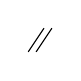
\begin{tikzpicture}[scale=0.2, baseline={([yshift=-0.5ex]current bounding box.center)}]  
			\draw[thin] (0,0) -- (1,1.5);  
			\draw[thin] (0.5,0) -- (1.5,1.5);  
		\end{tikzpicture}%  
	}%  
}  
\newcommand{\fourch}[4]
{\\[3pt]
	\begin{tabular}
		{*{4}{@{}p{4cm}}}
		A.~#1 & B.~#2 & C.~#3 & D.~#4
	\end{tabular}	
}
\newcommand{\fourchh}[4]
{\\[5pt]
	\begin{tabular}
		{*{4}{@{}p{20cm}}}
		A.~#1 \\[5pt] B.~#2 \\[5pt] C.~#3 \\[5pt] D.~#4
	\end{tabular}	
}
\newcommand{\fourchhh}[4]
{\\[3pt]
	\begin{tabular}
		{*{4}{@{}p{7.5cm}}}
		A.~#1 & B.~#2 \\[2pt] C.~#3 & D.~#4
	\end{tabular}	
}
\newcommand{\independent}{\perp\!\!\!\perp}
\everymath{\displaystyle}
\allowdisplaybreaks


\begin{document}

\pagestyle{fancy}
\lhead{Lecture 5}
\chead{illusion \& FzRainD}
\rhead{\today}

\setcounter{section}{4}

\section{向量组的极大线性无关组}

从本节开始,我们关注的重点从线性方程组的公式解转变到线性方程组解的结构,事实上我们已经有如下刻画:

\begin{theorem}[非齐次线性方程组解的结构] \label{5.0.1}
	设 \( A \in \F\mn, \; \beta \in \F^m \),给定非齐次线性方程组 \( AX=\beta \),且 \( r(A)=r(\overline{A})=r \). 那么存在 \( n-r(A)=:k \) 个自由未知量 \( c_1,\cdots,c_{k} \in \F \) 以及{\color{blue} 线性无关的} \( n \) 维列向量 \( \gamma,\eta_1,\cdots,\eta_k \in \F^n \),使得方程 \( AX=\beta \) 解的全体可以表示为
	\[ X=\gamma+c_1\eta_1+\cdots+c_k\eta_k. \] 
	
	其中要求 \( \gamma \) 为方程 \( AX=\beta \) 的一个特解,而 \( \eta_1,\cdots,\eta_k \) 为方程 \( AX=\bm{0} \) 的若干不同解.
\end{theorem}


\begin{corollary}[齐次线性方程组的解的结构] \label{5.0.2}
	设 \( A \in \F\mn, \; \beta \in \F^m \),给定齐次线性方程组 \( AX=\bm{0} \),且 \( r(A)=r \). 那么存在 \( n-r(A)=:k \) 个自由未知量 \( c_1,\cdots,c_{k} \in \F \) 以及{\color{blue} 线性无关的} \( n \) 维列向量 \( \eta_1,\cdots,\eta_k \in \F^n \),使得方程 \( AX=\bm{0} \) 解的全体可以表示为
	\[ X=c_1\eta_1+\cdots+c_k\eta_k. \] 
	
	其中 \( \eta_1,\cdots,\eta_k \) 为方程 \( AX=\bm{0} \) 的若干不同解.
\end{corollary}

定理 \ref{5.0.1} 告诉我们 \( AX=\beta \) 的解向量集合中存在 \( k+1 \) 个线性无关的向量,但是没有回答是否存在 \( k+2 \) 个或是更多的线性无关的向量? 另一方面,方程的任意解都可以被这 \( k+1 \) 个线性无关的向量的线性组合所表出,那么能否被更多或者更少个的线性无关向量所表出呢? 这就是本节我们需要回答的问题. 我们将从向量组的通用理论出发,研究线性方程组的向量组表达形式 \( x_1\alpha_1+\cdots+x_n\alpha_n=\beta \).

在后续讨论中,我们主要研究 \( n \) 维列向量,\( n \) 维行向量的结论完全平行,只需要在书写上稍加改变即可. 我们关注的向量集总是 \( \F^n \) 中由有限个向量组成的向量组,如果某个向量集中包含无限多个向量,称为向量族.

\subsection{回顾:向量组的线性关系}

在行列式的几何动机中我们已经接触过向量组的线性关系,这些概念是对 \( \R^2 \) 和 \( \R^3 \) 中共线,共面等概念在一般向量空间 \( \F^n \) 乃至更一般的线性空间 \( V \) 中的抽象化.

\subsubsection{线性关系及其性质}

\begin{definition}[线性关系]
	设 \( \alpha_1,\cdots,\alpha_s \in \F^n \),那么
	\begin{enumerate}[(1)]
		\item 称 \( \alpha_1,\cdots,\alpha_s \) 线性相关,若存在不全为零的 \( c_1,\cdots,c_s \in \F \) 使得 \( c_1\alpha_1+\cdots+c_s\alpha_s= \bm{0} \);
		\item 称 \( \alpha_1,\cdots,\alpha_s \) 线性无关,若对任意 \( c_1,\cdots,c_s \in \F \) 使得 \( c_1\alpha_1+\cdots+c_s\alpha_s= \bm{0} \) 都有 \( c_1=\cdots=c_s=0 \).
		\item 再给 \( \beta \in \F^n \),若存在 \( c_1,\cdots,c_s \in \F \) 使得 \( \beta= c_1\alpha_1+\cdots+c_s\alpha_s \) 成立,称 \( \beta \) 可由 \( \alpha_1,\cdots,\alpha_s \) 线性表出.
	\end{enumerate} 
\end{definition}

\begin{proposition} \label{5.1.2}
	设 \( \alpha_1,\cdots,\alpha_n \in \F^n-\{\bm{0}\} \),那么下列说法等价:
	\begin{enumerate}
		\item[(1)] \( \alpha_1,\cdots,\alpha_n \) 线性相关;
		\item[(2)] 存在 \( \alpha_t \; (1 \leq t \leq n) \) 可以由 \( \{\alpha_1,\cdots,\alpha_n\}-\{\alpha_t\} \) 线性表出;
		\item[{\color{red} (2')}] 存在 \( \alpha_t \; ({\color{red} 2} \leq t \leq n) \) 可以由 \( \alpha_1,\cdots,\alpha_{t-1} \) 线性表出;
		\item[(3)] 矩阵 \( A=(\alpha_1,\cdots,\alpha_n) \) 不可逆;
		\item[(4)] 若 \( \beta \in \F^n \) 可以由 \( \alpha_1,\cdots,\alpha_n \) 线性表出,那么表示法不唯一.
	\end{enumerate}
\end{proposition}

\begin{proof}
	(1) \( \Leftrightarrow \) (2). 设 \( \alpha_1,\cdots,\alpha_n \) 线性相关,故存在不全为零的数 \( c_1,\cdots,c_n \in \F \) 使 \( c_1\alpha_1+\cdots+c_n\alpha_n= \bm{0} \). 于是可以取到 \( c_t \neq 0 \; (1 \leq t \leq n) \). 那么
	\[ \alpha_t= -c_t^{-1} \sum_{i \neq t}^{} c_i\alpha_i= \sum_{i \neq t}^{} (-c_t^{-1}c_i) \alpha_i. \]
	
	反之,设 
	\[ \alpha_t=\sum_{i \neq t}^{} c_i\alpha_i \; (c_i \in \F) \leadsto \sum_{i=1}^{n} c_i\alpha_i=\bm{0} \; (c_t:=-1). \]
	
	显然 \( c_1,\cdots,c_n \) 不全为零.
	
	\vspace{1ex}
	
	(1) \( \Rightarrow \) (2'). 设 \( \alpha_1,\cdots,\alpha_n \) 线性相关,故存在不全为零的数 \( c_1,\cdots,c_n \in \F \) 使 \( c_1\alpha_1+\cdots+c_n\alpha_n= \bm{0} \). 现在取 \( t:=\max\{i: c_i \neq 0, 1 \leq i \leq n\} \). 断言 \( t \geq 2 \),否则 \( t=1 \) 蕴含
	\[ \sum_{i=1}^{n} c_i\alpha_i= c_1\alpha_1=\bm{0} \; (c_1 \neq 0) \leadsto \alpha_1=\bm{0}. \]
	
	与我们假设 \(\alpha_1 \in \F^n-\{\bm{0}\} \) 矛盾,那么 
	\[ \sum_{i=1}^{n} c_i\alpha_i=\sum_{i=1}^{t} c_i\alpha_i=\bm{0} \; (c_t \neq 0) \leadsto \alpha_t= \sum_{i=1}^{t-1} (-c_{t}^{-1}c_i)\alpha_i. \]
	
	(2') \( \Rightarrow \) (3). 设 \( \alpha_t=c_1\alpha_1+\cdots+c_{t-1}\alpha_{t-1} \; (c_i \in \F, 1\leq i \leq t-1) \). 由行列式的性质可知
	\[ \det A= \det(\alpha_1,\cdots,\alpha_{t-1},\alpha_t-(c_1\alpha_1+\cdots+c_{t-1}\alpha_{t-1}),\alpha_{t+1},\cdots,\alpha_n)=\det(\alpha_1,\cdots,\alpha_{t-1},\bm{0},\alpha_{t+1},\cdots,\alpha_n)=0. \]
	
	(3) \( \Rightarrow \) (4). 由  \( \beta \in \F^n \) 可以由 \( \alpha_1,\cdots,\alpha_n \) 线性表出,那么存在 \( c_1,\cdots,c_n \in \F \) 使得 
	\[ \beta=c_1\alpha_1+\cdots+c_n\alpha_n \leadsto A(c_1,\cdots,c_n)\T=:A\gamma_1=\beta. \]
	
	即 \( AX=\beta \) 有解 \( X=\gamma \). 又 \( A \) 不可逆,故 \( AX=\bm{0} \) 存在非零解 \( X=\eta \neq \bm{0} \),于是 \( X=\gamma+\eta \) 也是 \( AX=\beta \) 的一个解,且异于 \( \gamma \),这就给出了另一种表示系数.
	
	(4) \( \Rightarrow \) (1). 设 
	\[ \beta=\sum_{i=1}^{n} c_i\alpha_i= \sum_{i=1}^{n} d_i\alpha_i, \; c_i,d_i \in \F \]
	
	为两种不同的表示法,那么存在 \( 1 \leq t \leq n \),使得 \( c_t \neq d_t \). 于是
	\[ \sum_{i=1}^{n} (c_i-d_i)\alpha_i= \bm{0} \]
	
	前面的系数不全为零.
	
\end{proof}

\begin{corollary} \label{5.1.3}
	设 \( \alpha_1,\cdots,\alpha_n \in \F^n \),那么下列说法等价:
	\begin{enumerate}[(1)]
		\item \( \alpha_1,\cdots,\alpha_n \) 线性无关;
		\item 矩阵 \( A=(\alpha_1,\cdots,\alpha_n) \) 可逆;
		\item 若 \( \beta \in \F^n \) 可以由 \( \alpha_1,\cdots,\alpha_n \) 线性表出,那么表示法唯一.
	\end{enumerate}
\end{corollary}

命题 \ref{5.1.2} (3) 和推论 \ref{5.1.3} (2) 给出了判断 {\color{red} \( n \) 个 \( n \) 维向量}组成的向量组线性相关和无关的一种比较简洁的方法,可以转化为求向量组拼成矩阵的行列式. 对于一般个数的向量组来说,还是要归结于求解线性方程组.

\begin{example}
	已知 \( \alpha_1=(1,0,2,3)\T, \alpha_2=(1,1,3,5)\T, \alpha_3=(1,-1,2+a,1)\T, \alpha_4=(1,2,4,8+a)\T \) 以及 \( \beta=(1,1,3+b,5)\T \). 试讨论
	\begin{enumerate}[(1)]
		\item \(a,b \) 为何值时,\( \beta \) 不能表示为 \( \alpha_1,\alpha_2,\alpha_3,\alpha_4 \) 的线性组合;
		\item \(a,b \) 为何值时,\( \beta \) 可由 \( \alpha_1,\alpha_2,\alpha_3,\alpha_4 \) 唯一线性表出,并写出表示法;
		\item \(a,b \) 为何值时,\( \beta \) 可由 \( \alpha_1,\alpha_2,\alpha_3,\alpha_4 \) 线性表出,但表示法不唯一. 并写出所有的表示法.
	\end{enumerate}
\end{example}

\begin{solution}
	设 \( A=(\alpha_1,\cdots,\alpha_4) \). 那么 \( \beta \) 可以表示为 \( \alpha_1,\alpha_2,\alpha_3,\alpha_4 \) 的线性组合等价于 \( AX=\beta \) 有解,也即 \( r(A)=r(\overline{A})=r(A,\beta) \). 下面对增广矩阵 \( \overline{A} \) 实行初等行变换
	\[ \begin{bNiceMatrix}
		1 & 1 & 1 & 1 & \Vdots & 1 \\
		0 & 1 & -1 & 2 & & 1 \\
		2 & 3 & 2+a & 4 & & 3+b \\
		3 & 5 & 1 & 8+a & & 5 
	\end{bNiceMatrix} \leadsto \begin{bNiceMatrix}
	1 & 1 & 1 & 1 & \Vdots & 1 \\
	0 & 1 & -1 & 2 & & 1 \\
	0 & 1 & a & 2 & & 1+b \\
	0 & 2 & -2 & 5+a & & 2 
	\end{bNiceMatrix} \leadsto \begin{bNiceMatrix}
	1 & 1 & 1 & 1 & \Vdots & 1 \\
	0 & 1 & -1 & 2 & & 1 \\
	0 & 0 & 1+a & 0 & & b \\
	0 & 0 & 0 & 1+a & & 0 
	\end{bNiceMatrix}.  \]
	
	(1) 若 \( 1+a=0, \; b \neq 0 \),那么 \( r(A)=2, \; r(\overline{A})=r(A,\beta)=3 \). 即 \( AX=\beta \) 无解,故 \( \beta \) 不能表示为 \( \alpha_1,\alpha_2,\alpha_3,\alpha_4 \) 的线性组合.
	
	(2) 若 \( 1+a \neq 0 \),那么  \( r(A)=r(\overline{A})=r(A,\beta)=4 \). 这时,\( A=(\alpha_1,\cdots,\alpha_4) \) 显然可逆,故 \( \beta \) 可由 \( \alpha_1,\alpha_2,\alpha_3,\alpha_4 \) 唯一线性表出. 为求表示法,继续对上述矩阵实行初等行变换
	\[ \begin{bNiceMatrix}
		1 & 1 & 1 & 1 & \Vdots & 1 \\
		0 & 1 & -1 & 2 & & 1 \\
		0 & 0 & 1+a & 0 & & b \\
		0 & 0 & 0 & 1+a & & 0 
	\end{bNiceMatrix} \leadsto \begin{bNiceMatrix}
	1 & 0 & 0 & 0 & \Vdots & (-2b)/(1+a) \\
	0 & 1 & 0 & 0 & & (1+a+b)/(1+a) \\
	0 & 0 & 1 & 0 & & b/(1+a) \\
	0 & 0 & 0 & 1 & & 0 
	\end{bNiceMatrix}.  \]
	
	于是
	\[ \beta= \left(-\frac{2b}{1+a}\right) \alpha_1+ \left(\frac{1+a+b}{1+a}\right) \alpha_2+ \left(\frac{b}{1+a}\right) \alpha_3+ 0 \cdot \alpha_4. \]
	
	(3) 若 \( 1+a=b=0 \),那么 \( r(A)=r(\overline{A})=r(A,\beta)=2 \). 这时,\( A=(\alpha_1,\cdots,\alpha_4) \) 显然不可逆,故 \( \beta \) 可由 \( \alpha_1,\alpha_2,\alpha_3,\alpha_4 \) 线性表出,但表示法不唯一.
	
	\[ \begin{bNiceMatrix}
		1 & 1 & 1 & 1 & \Vdots & 1 \\
		0 & 1 & -1 & 2 & & 1 \\
		0 & 0 & 1+a & 0 & & b \\
		0 & 0 & 0 & 1+a & & 0 
	\end{bNiceMatrix}=\begin{bNiceMatrix}
	1 & 1 & 1 & 1 & \Vdots & 1 \\
	0 & 1 & -1 & 2 & & 1 \\
	0 & 0 & 0 & 0 & & 0 \\
	0 & 0 & 0 & 0 & & 0 
	\end{bNiceMatrix} \leadsto \begin{bNiceMatrix}
	1 & 0 & 2 & -1 & \Vdots & 0 \\
	0 & 1 & -1 & 2 & & 1 \\
	0 & 0 & 0 & 0 & & 0 \\
	0 & 0 & 0 & 0 & & 0 
	\end{bNiceMatrix}.  \]
	
	那么 \( AX=\beta \) 的解可以写为
	\[ X=\begin{bmatrix}
		0 \\ 1 \\ 0 \\ 0
	\end{bmatrix}+ x_3\begin{bmatrix}
	-2 \\ 1 \\ 1 \\ 0
	\end{bmatrix}+x_4\begin{bmatrix}
	1 \\ -2 \\ 0 \\ 1
	\end{bmatrix}, \; x_3,x_4 \in \F. \]
	
	即
	\[ \beta=(-2x_3+x_4) \alpha_1+(1+x_3-2x_4)\alpha_2+x_3 \cdot \alpha_3+x_4 \cdot \alpha_4, \; x_3,x_4 \in \F. \]
\end{solution}

下面介绍两个简单的命题,提供了一种判断线性相关性的方法:对原向量组进行扩充或截短.

\begin{proposition} \label{5.1.5}
	设 \( \alpha_1,\cdots,\alpha_s \in \F^n \),以及 \( t \leq n \),那么
	\begin{enumerate}[(1)]
		\item 若 \( \alpha_1,\cdots,\alpha_t \) 线性相关,那么 \( \alpha_1,\cdots,\alpha_s \) 线性相关,即部分相关则整体相关;
		\item 若 \( \alpha_1,\cdots,\alpha_s \) 线性无关,那么 \( \alpha_1,\cdots,\alpha_t \) 线性无关,即整体无关则部分无关.
	\end{enumerate}
\end{proposition}

\begin{proof}
	注意到 (2) 为 (1) 的逆否命题,正确性相同,故只证明 (1). 由于  \( \alpha_1,\cdots,\alpha_t \) 线性相关,那么存在不全为零的 \( c_1,\cdots,c_t \in \F \) 使得 
	\[ c_1\alpha_1+\cdots+c_t\alpha_t=c_1\alpha_1+\cdots+c_t\alpha_t+0\cdot \alpha_{t+1}+\cdots+0 \cdot \alpha_n=\bm{0}. \]
\end{proof}

\begin{proposition} \label{5.1.6}
	设 \( \alpha_1,\cdots,\alpha_s \in \F^n \),以及 \( m \leq n \),现在截取 \( \alpha_1,\cdots,\alpha_s \) 的前 \( m \) 行分量组成新向量组 \( \widetilde{\alpha}_1,\cdots,\widetilde{\alpha}_s \in \F^m \),那么
	\begin{enumerate}[(1)]
		\item 若 \( \widetilde{\alpha}_1,\cdots,\widetilde{\alpha}_s \) 线性无关,那么 \( \alpha_1,\cdots,\alpha_s \) 线性无关;
		\item 若 \( \alpha_1,\cdots,\alpha_s \) 线性相关,那么 \( \widetilde{\alpha}_1,\cdots,\widetilde{\alpha}_s \) 线性相关.
	\end{enumerate}
\end{proposition}

\begin{proof}
	注意到 (2) 为 (1) 的逆否命题,正确性相同,故只证明 (1). 考虑 \( \F\)-线性组合 \( c_1\alpha_1+\cdots+c_s\alpha_s=\bm{0} \),这事实上是一个关于 \( s \) 个变元的 \( n \) 个方程组成的线性方程组 (I),取方程组 (I) 的前 \( m \) 行组成的子方程组 (II),显然 (I) 的解必定为 (II) 的解. 但由于 \( \widetilde{\alpha}_1,\cdots,\widetilde{\alpha}_s \) 线性无关,故 (II) 只有零解,进而 (I) 也只有零解,即 \( \alpha_1,\cdots,\alpha_s \) 线性无关.
\end{proof}

\begin{example}
	设 \( \F \) 为数域,\( \alpha_i:=(1,t_i,t_i^2,\cdots,t_i^{n-1})\T, \; i=1,2,\cdots,r \). 其中 \( t_1,\cdots,t_r \in \F \) 为互不相同的数且 \( r \leq n \),证明 \( \alpha_1,\cdots,\alpha_r \) 线性无关.
\end{example}

\begin{proof}
	(\textbf{法一})\ 考虑 \( \alpha_i \) 的前 \( r \) 行分量组成的截短组 \( \widetilde{\alpha}_i:=(1,t_i,t_i^2,\cdots,t_i^{r-1})\T \),由推论 \ref{5.1.3} (2) 可知
	\[ \det \begin{bmatrix}
	     1 & 1 & \cdots & 1 \\
	     t_1 & t_2 & \cdots & t_{r} \\
	     \vdots & \vdots & \ddots & \vdots \\
	     t_1^{r-1} & t_2^{r-1} & \cdots & t_{r}^{r-1}
	\end{bmatrix}= \prod_{1 \leq i <j \leq r}^{} (t_i-t_j) \neq 0 \leadsto \{\widetilde{\alpha}_i\}_{1 \leq i \leq r} \; \text{linearly independent.} \]
	
	由命题 \ref{5.1.6} (1) 即证.
	
	(\textbf{法二})\ 取 \( t_{r-1},\cdots,t_n \in \F-\{t_1,\cdots,t_r\} \) 互不相同,由于 \( \F \) 为数域(无限域),这总能做到. 补充定义 \( \alpha_i:=(1,t_i,t_i^2,\cdots,t_i^{n-1})\T, \; i=r+1,\cdots,n \). 同法一可知 \( \alpha_1,\cdots,\alpha_n \) 线性无关,再由命题 \ref{5.1.5} (2) 即证.
\end{proof}

\begin{proposition} \label{5.1.8}
	设 \( \alpha_1,\cdots,\alpha_s \in \F^n \) 线性无关,且 \( \alpha_1,\cdots,\alpha_s, \beta \in \F^n \) 线性相关,那么 \( \beta \) 可以由 \( \alpha_1,\cdots,\alpha_s \) 唯一线性表出.
\end{proposition}

\begin{proof}
	由推论 \ref{5.1.3} (3) 只需证 \( \beta \) 可以由 \( \alpha_1,\cdots,\alpha_s \) 线性表出. 由于  \( \alpha_1,\cdots,\alpha_s, \beta \in \F^n \) 线性相关,那么存在一组不全为零的数 \( c_1,\cdots,c_s,c_{s+1} \in \F \) 使
	\[ c_1\alpha_1+c_2\alpha_2+\cdots+c_s\alpha_s+c_{s+1}\beta=\bm{0}. \]
	
	断言 \( c_{s+1} \neq 0 \),否则 \( c_1\alpha_1+c_2\alpha_2+\cdots+c_s\alpha_s=\bm{0} \),再由  \( \alpha_1,\cdots,\alpha_s \in \F^n \) 线性无关可知 \( c_1=\cdots=c_s=0 \),这与 \( c_1,\cdots,c_s,c_{s+1} \) 不全为零矛盾. 于是
	\[ \beta= \sum_{i=1}^{n} (-c_{s+1}^{-1}c_i)\alpha_i. \]
	
\end{proof}


\begin{example}
	设向量组 \( \alpha_1,\cdots,\alpha_{s-1} \; (s \geq 3) \) 线性相关,向量组 \( \alpha_2,\cdots,\alpha_s \) 线性无关,问:
	\begin{enumerate}[(1)]
		\item \( \alpha_1 \) 能否由 \( \alpha_2,\cdots,\alpha_{s-1} \) 线性表出?
		\item \( \alpha_s \) 能否由 \( \alpha_1,\cdots,\alpha_{s-1} \) 线性表出?
	\end{enumerate}
\end{example}

\begin{solution}
	(1) 由命题 \ref{5.1.5} (2) 可知 \( \alpha_2,\cdots,\alpha_{s-1} \) 线性无关,再由命题 \ref{5.1.8} 可知 \( \alpha_1 \) 可由 \( \alpha_2,\cdots,\alpha_{s-1} \) 线性表出,且表示法唯一.
	
	(2) 若存在 \( c_1,\cdots,c_{s-1} \in \F \) 使得 \( \alpha_s=c_1\alpha_1+\cdots+c_{s-1}\alpha_{s-1} \). 由 (1) 知存在 \( d_2,\cdots,d_{s-1} \in \F \) 使得 \( \alpha_1=d_2\alpha_2+\cdots+d_{s-1}\alpha_{s-1} \). 于是
	\[ \alpha_s= \sum_{i=2}^{s-1} (c_i+c_1d_i) \alpha_i \leadsto \sum_{i=2}^{s-1} (c_i+c_1d_i) \alpha_i-\alpha_s=\bm{0}. \]
	
	显然这个 \( \F\)-线性组合中 \( \alpha_s \) 前系数非零,推知 \( \alpha_2,\cdots,\alpha_s \) 线性相关,导出矛盾. 故 \( \alpha_s \) 不能由 \( \alpha_1,\cdots,\alpha_{s-1} \) 线性表出.
	
\end{solution}

\subsubsection{线性表出与矩阵}

在上一小节的讨论中,我们主要关注的是一个向量组内部的线性关系,并尝试将一个向量能由一个向量组线性表出转化为线性方程组的语言. 在本小节,我们开始研究两个向量组之间的关系.

\begin{definition}[向量组的线性表出]
	给定向量组 (I): \( \{\alpha_1,\cdots,\alpha_s\} \subseteq \F^n \),(II): \( \{\beta_1,\cdots,\beta_t\} \subseteq \F^n \). 若对每个 \( \alpha_i \; (1 \leq i \leq s) \),\( \alpha_i \) 都能由向量组 (II) 线性表出,则称向量组 (I) 能被向量组 (II) 线性表出.
\end{definition}

\begin{proposition} \label{5.1.11}
	给定向量组 (I): \( \{\alpha_1,\cdots,\alpha_s\} \subseteq \F^n \),(II): \( \{\beta_1,\cdots,\beta_t\} \subseteq \F^n \),那么下列叙述等价:
	\begin{enumerate}[(1)]
		\item 向量组 (I) 能被向量组 (II) 线性表出;
		\item 记 \( A=(\alpha_1,\cdots,\alpha_s), \; B=(\beta_1,\cdots,\beta_t) \),那么存在矩阵 \( C \in \F^{t \times s} \),使得 \( A=BC \);
		\item 记 \( M=(\alpha_1\T,\cdots,\alpha_s\T)\T, \; N=(\beta_1\T,\cdots,\beta_t\T)\T \),那么存在矩阵 \( L \in \F^{s \times t} \),使得 \( M=LN \).
	\end{enumerate}
\end{proposition}

\begin{proof}
    若向量组 (I) 能被向量组 (II) 线性表出,那么设
    \[ \left\{ \begin{array}{l}
    	\alpha_1=c_{11}\beta_1+c_{{\color{red} 21}}\beta_2+\cdots+c_{t1}\beta_t, \\
    	\alpha_2=c_{{\color{red} 12}}\beta_1+c_{22}\beta_2+\cdots+c_{t2}\beta_t, \\
    	\cdots\cdots \\
    	\alpha_s=c_{1s}\beta_1+c_{2s}\beta_2+\cdots+c_{ts}\beta_t.
    \end{array}\right. \leadsto (\alpha_1,\cdots,\alpha_s)=(\beta_1,\cdots,\beta_t)\begin{bmatrix}
     c_{11} & c_{12} & \cdots & c_{1s} \\
     c_{21} & c_{22} & \cdots & c_{2s} \\
     \vdots & \vdots & \ddots & \vdots \\
     c_{t1} & c_{t2} & \cdots & c_{ts}
    \end{bmatrix} (*) \]
    
    这就找到了 \( C=(c_{ij}) \),对 \( (*) \) 取转置得到
    \[ \begin{bmatrix}
    	\alpha_1\T \\
    	\alpha_2\T \\
    	\vdots \\
    	\alpha_s\T
    \end{bmatrix}=\begin{bmatrix}
    c_{11} & c_{21} & \cdots & c_{t1} \\
    c_{12} & c_{22} & \cdots & c_{t2} \\
    \vdots & \vdots & \ddots & \vdots \\
    c_{1s} & c_{2s} & \cdots & c_{ts}
    \end{bmatrix}\begin{bmatrix}
    \beta_1\T \\
    \beta_2\T \\
    \vdots \\
    \beta_s\T
    \end{bmatrix}. \]
    
    这就找到了 \( L=(c_{ji}) \),上面的推理都可以逆向进行,故等价性成立.
\end{proof}

\begin{corollary} \label{5.1.12}
	给定矩阵 \( A \in \F\nm, \; B \in \F\nm \),那么
	\begin{enumerate}[(1)]
		\item ({\color{blue}\textbf{“左行”}}) \( A \) 的行向量组可以被 \( B \) 的行向量组线性表出 \( \Leftrightarrow \) 存在 \( C \in \F\n \),使得 \( A=CB \);
		\item ({\color{blue}\textbf{“右列”}}) \( A \) 的列向量组可以被 \( B \) 的列向量组线性表出 \( \Leftrightarrow \) 存在 \( D \in \F^{m \times m} \),使得 \( A=BD \).
	\end{enumerate}
\end{corollary}

\begin{proposition} \label{5.1.13}
	给定向量组 (I): \( \{\alpha_1,\cdots,\alpha_s\} \subseteq \F^n \),(II): \( \{\beta_1,\cdots,\beta_t\} \subseteq \F^n \),且向量组 (I) 能被向量组 (II) 线性表出. 
	\begin{enumerate}[(1)]
		\item \( s>t \),则 \( \alpha_1,\cdots,\alpha_s \) 必定线性相关;
		\item 若 \( \alpha_1,\cdots,\alpha_s \) 线性无关,那么 \( s \leq t \).
	\end{enumerate}
\end{proposition}

\begin{proof}
	只验证 (1). 取 \( \F\)-线性组合 \( a_1\alpha_1+\cdots+a_s\alpha_s=\bm{0} \). 由命题 \ref{5.1.11} (2) 可知存在矩阵 \( C=(c_{ij}) \in \F^{t \times s} \) 使得 \( (\alpha_1,\cdots,\alpha_s)=(\beta_1,\cdots,\beta_t)C \). 令 \( X=(a_1,\cdots,a_s)\T \),断言 
	\begin{equation}
		\bm{0}=(\alpha_1,\cdots,\alpha_s)X={\color{red} [(\beta_1,\cdots,\beta_t)C]X=(\beta_1,\cdots,\beta_t)(CX)}.
		\label{5.1.13.1}
	\end{equation}
	
	(\textbf{法一})\ 向量组 (I) (II) 均为 \( \F^n \) 中向量,每个分量都是 \( \F \) 中的数,那么 \( (\alpha_1,\cdots,\alpha_s), (\beta_1,\cdots,\beta_t) \) 就是某个矩阵的按列分块形式写法,这里的结合律直接继承矩阵的结合律得到.
	
	(\textbf{法二})\ 将向量组 (I) (II) 均视为抽象的向量,\( (\alpha_1,\cdots,\alpha_s)X:=c_1\alpha_1+\cdots+c_s\alpha_s \) 并不是矩阵乘法.而是方便起见我们给予的一种形式上的记号. 按照该定义验证:
	\[ [(\beta_1,\cdots,\beta_t)C]X=\left( \sum_{i=1}^{t} c_{i1}\beta_i, \sum_{i=1}^{t} c_{i2}\beta_i, \cdots, \sum_{i=1}^{t} c_{is}\beta_i \right)X= \sum_{j=1}^{s} a_j \left( \sum_{i=1}^{t} c_{ij}\beta_i \right)= \sum_{i=1}^{t}\left( \sum_{j=1}^{s} c_{ij}a_j \right) \beta_i. \]
	
	\[ (\beta_1,\cdots,\beta_t)(CX)=\sum_{i=1}^{t} (CX)_i \beta_i= \sum_{i=1}^{t}\left( \sum_{j=1}^{s} c_{ij}a_j \right) \beta_i. \]
	
	也就说明这种形式上的记号满足结合律,我们在第三章研究线性空间时会继续用到这个结果.
	
	接下来为了找到不全为零的 \( a_1,\cdots,a_s \),只需要找到一个非零的 \( X \in \F^s \) 满足 (\ref{5.1.13.1}) 式即可. 不妨考察线性方程组 \( CX=\bm{0} \),这里的未知量总数为 \( s \),但 \( r(C) \leq \min\{t,s\}=t<s \),于是由推论 \ref{5.0.2} 可知存在 \( s-t \) 个线性无关的解向量 \( \eta_1,\cdots,\eta_{s-t} \),任取其中之一即为我们所求非零的 \( X \in \F^s \).
	
\end{proof}


\begin{corollary} \label{5.1.14}
	设 \( \alpha_1,\cdots,\alpha_s \in \F^n, \; A:=(a_{ij}) \in \F^{s \times t}, \; X=(c_1,\cdots,c_s)\T \in \F^{t}, \; B \in \F^{t \times p} \),引入如下的形式记号
	\[ (\alpha_1,\cdots,\alpha_s)X:=c_1\alpha_1+\cdots+c_s\alpha_s, \; (\alpha_1,\cdots,\alpha_s)A:=\left( \sum_{i=1}^{s} a_{i1}\alpha_1, \cdots, \sum_{i=1}^{s} a_{i1}\alpha_t \right). \]
	
	这样的形式记号满足运算性质:
	\begin{enumerate}[(1)]
		\item \( [(\alpha_1,\cdots,\alpha_s)A]X=(\alpha_1,\cdots,\alpha_s)(AX) \);
		\item \( [(\alpha_1,\cdots,\alpha_s)A]B=(\alpha_1,\cdots,\alpha_s)(AB) \).
	\end{enumerate}
\end{corollary}


\begin{proof} 
	模仿命题 \ref{5.1.13} 的证明过程即可,当然你也可以直接将 \( (\alpha_1,\cdots,\alpha_s) \) 视作 \( \F^{n \times s} \) 矩阵,然后用矩阵的结合律,不过命题 \ref{5.1.13} 的法二更具有一般性,即使这里的 \( \alpha_i \) 是抽象的向量也是可行的.
\end{proof}


\begin{corollary} \label{5.1.15}
	设 \( \alpha_1,\cdots,\alpha_{n+1} \in \F^n \),那么 \( \alpha_1,\cdots,\alpha_{n+1} \) 必然线性相关.
\end{corollary}

\begin{proof}
	只需要注意到向量组 \( \alpha_1,\cdots,\alpha_{n+1} \) 必然能被向量组 \( \varepsilon_1, \varepsilon_2, \cdots, \varepsilon_n \) 线性表出,且 \( n+1>n \),利用命题 \ref{5.1.13} (1) 即得.
\end{proof}

\begin{practice} \label{prac5.1}
	给定向量组 (I): \( \{\alpha_1,\cdots,\alpha_s\} \subseteq \F^n \),(II): \( \{\beta_1,\cdots,\beta_t\} \subseteq \F^n \),且向量组 (I) 能被向量组 (II) 线性表出,即存在矩阵 \( C=(c_{ij}) \in \F^{t \times s} \) 使得 \( (\alpha_1,\cdots,\alpha_s)=(\beta_1,\cdots,\beta_t)C \). 现设 \( \beta_1,\cdots,\beta_t \) 线性无关. 证明:
	\begin{enumerate}[(1)]
		\item \( \alpha_1,\cdots,\alpha_s \) 线性无关的充分必要条件为 \( C \) 列满秩,即 \( r(C)=s \);
		\item 特别地,当 \( s=t \) 时,\( \alpha_1,\cdots,\alpha_s \) 线性无关的充分必要条件为 \( C \) 可逆.
	\end{enumerate}
\end{practice}

\begin{proof}
	只证明 (1). 考虑 \( \F\)-线性组合 \( a_1\alpha_1+\cdots+a_s\alpha_s=\bm{0} \). 设 \( X=(a_1,\cdots,a_s)\T \),由推论 \ref{5.1.14} 可知
	\[ (\alpha_1,\cdots,\alpha_s)X=(\beta_1,\cdots,\beta_t)CX=\bm{0}. \]
	
	由于 \( \beta_1,\cdots,\beta_t \) 线性无关,只能 \( CX=\bm{0} \). 下面断言 \( CX=\bm{0} \) 仅有零解的充分必要条件为 \( C \) 列满秩. 一方面,当 \( C \) 列满秩时,\( C \) 存在左逆 \( K \),那么 \( X=(KC)X=K(CX)=O \). 另一方面,当 \( C \) 非列满秩时,由推论 \ref{5.0.2} 可知存在 \( s-r(C)>0 \) 个线性无关的解向量,任取其中之一都是一个非零解.
	 
\end{proof}


\begin{example} \label{5.1.16}
	设 \( \alpha_1,\cdots,\alpha_n \in \F^n \) 线性无关,判断下列构造的 \( \beta_1,\cdots,\beta_n \in \F^n \) 的线性相关性.
	\begin{enumerate}[(1)]
		\item \( \beta_i=\alpha_1+\cdots+\alpha_i \; (1 \leq i \leq n) \);
		\item \( \beta_i=\alpha_i+\alpha_{i+1} \; (1 \leq i \leq n-1), \; \beta_n=\alpha_n+\alpha_1 \).
	\end{enumerate}
\end{example}

\begin{solution}
	注意到向量组 \( \beta_1,\cdots,\beta_n \) 可以由向量组  \( \alpha_1,\cdots,\alpha_n \) 线性表出,考虑利用练习 \ref{prac5.1}. 先考虑 (1).
	
	\[ (\beta_1,\cdots,\beta_n)=(\alpha_1,\cdots,\alpha_n)\begin{bmatrix}
		1 & 1 & 1 & \cdots & 1 \\
		0 & 1 & 1 & \cdots & 1 \\
		0 & 0 & 1 & \cdots & 1 \\
		\vdots & \vdots & \vdots & \ddots & \vdots \\
		0 & 0 & 0 & \cdots & 1
	\end{bmatrix}=:(\alpha_1,\cdots,\alpha_n)C. \]
	
	显然 \( \det C =1 \neq 0 \),,故 \( C \) 可逆,那么 \( \beta_1,\cdots,\beta_n \) 线性无关. 下面考虑 (2).
	
	\[ (\beta_1,\cdots,\beta_n)=(\alpha_1,\cdots,\alpha_n)\begin{bmatrix}
	1 & 0 & 0 & \cdots & 0 & 1 \\
	1 & 1 & 0 & \cdots & 0 & 0 \\
	0 & 1 & 1 & \cdots & 0 & 0 \\
	\vdots & \vdots & \vdots & \ddots & \vdots & \vdots \\
	0 & 0 & 0 & \cdots & 1 & 0 \\
	0 & 0 & 0 & \cdots & 1 & 1
	\end{bmatrix}=:(\alpha_1,\cdots,\alpha_n)C. \]
	
	求解下面的行列式,按第一行展开,
	\[ \det C= \begin{vmatrix}
		1 & 0 & 0 & \cdots & 0 & 1 \\
		1 & 1 & 0 & \cdots & 0 & 0 \\
		0 & 1 & 1 & \cdots & 0 & 0 \\
		\vdots & \vdots & \vdots & \ddots & \vdots & \vdots \\
		0 & 0 & 0 & \cdots & 1 & 0 \\
		0 & 0 & 0 & \cdots & 1 & 1
	\end{vmatrix}= 1+(-1)^{n+1}. \]
	
	当 \( n \) 为奇数时,\( \det C=2 \neq 0 \),那么 \( \beta_1,\cdots,\beta_n \) 线性无关; 当 \( n \) 为偶数时,\( \det C=0 \),蕴含 \( \beta_1,\cdots,\beta_n \) 线性相关. 
	
	
	
\end{solution}


\begin{definition}[向量组的等价]
	给定向量组 (I): \( \{\alpha_1,\cdots,\alpha_s\} \subseteq \F^n \),(II): \( \{\beta_1,\cdots,\beta_t\} \subseteq \F^n \). 称向量组 (I) 和向量组 (II) 等价,若向量组 (I) 和向量组 (II) 可以相互线性表出.
\end{definition}


\begin{proposition} \label{5.1.18}
	向量组的等价是一种等价关系.
\end{proposition}


\begin{proof}
	反身性和对称性是显然的. 对传递性. 取向量组 (I): \( \{\alpha_1,\cdots,\alpha_s\} \subseteq \F^n \),(II): \( \{\beta_1,\cdots,\beta_t\} \subseteq \F^n \),(III): \( \{\gamma_1,\cdots,\gamma_p\} \subseteq \F^n \),并设向量组 (I) 和向量组 (II) 等价,向量组 (II) 和向量组 (III) 等价,下证向量组 (I) 和向量组 (III) 等价. 由命题 \ref{5.1.11},存在矩阵 \( A_1 \in \F^{t \times s}, A_2 \in \F^{s \times t}, B_1 \in \F^{p \times t}, B_2 \in \F^{t \times p} \),使得
	\[ (\alpha_1,\cdots,\alpha_s)=(\beta_1,\cdots,\beta_t)A_1, \; (\beta_1,\cdots,\beta_t)=(\gamma_1,\cdots,\gamma_p)B_1. \]
	\[ (\beta_1,\cdots,\beta_t)=(\alpha_1,\cdots,\alpha_s)A_2, \; (\gamma_1,\cdots,\gamma_p)=(\beta_1,\cdots,\beta_t)B_2. \]
	
	利用推论 \ref{5.1.14} 得到 
	\[ (\alpha_1,\cdots,\alpha_s)=(\gamma_1,\cdots,\gamma_p)(B_1A_1), \; (\gamma_1,\cdots,\gamma_p)=(\alpha_1,\cdots,\alpha_s)(A_2B_2). \]
	
	再由命题 \ref{5.1.11},这就说明向量组 (I) 和向量组 (III) 可以相互线性表出,即向量组 (I) 和向量组 (III) 等价.
\end{proof}


\begin{example}
	取例 \ref{5.1.16} (1) 中的向量组 \( \{\alpha_1,\cdots,\alpha_n\} \) 以及 \( \{\beta_1,\cdots,\beta_n\} \),这里 \( \alpha_1,\cdots,\alpha_n \in \F^n \) 线性无关且 \( \beta_i=\alpha_1+\cdots+\alpha_i \; (1 \leq i \leq n) \),取
	\[ C=\begin{bmatrix}
		1 & 1 & 1 & \cdots & 1 \\
		0 & 1 & 1 & \cdots & 1 \\
		0 & 0 & 1 & \cdots & 1 \\
		\vdots & \vdots & \vdots & \ddots & \vdots \\
		0 & 0 & 0 & \cdots & 1
	\end{bmatrix}, \]
	
	那么 \( (\beta_1,\cdots,\beta_n)=(\alpha_1,\cdots,\alpha_n)C, \; (\beta_1,\cdots,\beta_n)C^{-1}=(\alpha_1,\cdots,\alpha_n)(CC^{-1})=(\alpha_1,\cdots,\alpha_n) \). 也就说明这两个向量组等价.
\end{example}

\begin{lemma} \label{5.1.20}
	给定向量组 (I): \( \{\alpha_1,\cdots,\alpha_s\} \subseteq \F^n \),(II): \( \{\beta_1,\cdots,\beta_t\} \subseteq \F^n \). 若向量组 (I) 和向量组 (II) 均为线性无关向量组且等价,那么 \( s=t \).
\end{lemma}

\begin{proof}
	由命题 \ref{5.1.13} (2) 可知,由于 \( \alpha_1,\cdots,\alpha_s \) 线性无关且向量组 (I) 能被向量组 (II) 线性表出,故 \( s \leq t \). 同理有 \( s \geq t \),于是 \( s=t \).
\end{proof}

\subsection{极大线性无关组和向量组的秩}

在前一小节,我们研究了一个有限向量组内部的线性关系,以及不同向量组之间的线性表出. 本小节中,我们聚焦于一个向量组中的核心部分,即整个向量组被它的部分组向量所线性表出的可能性及其性质。

\begin{example} \label{5.2.1}
	取 \( \alpha,\beta \in \mathbb{R}^2 \) 不共线,由平面向量基本定理知道,\( \mathbb{R}^2 \) 中的向量均可被 \( \alpha, \beta \) 唯一线性表出. 任取 \( \alpha_1,\cdots,\alpha_s \in \mathbb{R}^2-\{ \alpha, \beta \} \),显然向量组 \( \{\alpha,\beta\} \) 可以被向量组 \( \{\alpha, \beta,\alpha_1,\cdots,\alpha_s\} \) 线性表出,反之亦然,这就说明了 \( \{\alpha, \beta,\alpha_1,\cdots,\alpha_s\} \) 与 \( \{\alpha,\beta\} \) 等价.
\end{example}

例 \ref{5.2.1} 找到了一个向量组的部分组和整个向量组等价,也就说明我们想要研究整个向量组,只需要归结到研究这个部分组即可. 这样的部分组的选取也不是唯一的,如果存在 \( \alpha_i \; (1\leqslant i \leq s) \) 使得 \( \alpha_i, \beta \) 不共线,那么 \( \{\alpha_i,\beta\} \) 也可以充当这样与整个向量组等价的部分组. 为此,我们引入极大线性无关组的概念.

\begin{definition}[极大线性无关组] \label{5.2.2}
	设 \( S \subseteq \F^n \) 为一个向量集(可以是有限或无限多个向量),且存在一个向量组 \( \{\alpha_1,\cdots,\alpha_r\} \in S \) 满足:
	\begin{enumerate}[(1)]
		\item \( \alpha_1,\cdots,\alpha_r \) 线性无关;
		\item 向量集 \( S \) 中的任意向量可由 \( \alpha_1,\cdots,\alpha_r \) 线性表出;
		\item[{\color{red} (2')}] 将向量集 \( S \) 中任意向量添加到 \( \alpha_1,\cdots,\alpha_r \) 中得到的 \( r+1 \) 个向量线性相关,
	\end{enumerate}
	则称 \( \alpha_1,\cdots,\alpha_r \) 为向量集 \( S \) 的一个极大线性无关组,或简称极大无关组.
\end{definition}

\begin{remark}
	由推论 \ref{5.1.3} (3) 知道定义 \ref{5.2.2} (2) 中的线性表出,也可以修改为{\color{red}唯一}线性表出. 由于一个向量 \( \alpha \) 是线性相关的当且仅当 \( \alpha=\bm{0} \),于是仅由零向量组成的向量集没有极大线性无关组.
\end{remark}

\subsubsection{极大线性无关组的存在性}

在讨论极大线性无关组的性质前,我们自然会问这样定义的合理性,即任何一个向量集(可以是有限或者无限多个向量)是否必定存在一个部分组作为它的极大线性无关组呢? 我们先研究向量组的情形.

\begin{theorem}[向量组中的存在性]
	设 \( S \subseteq \F^n \) 为由有限个不全为零的向量所组成的向量组,那么 \( S \) 必定存在一个极大线性无关组.
\end{theorem}

\begin{proof}
	设 \( S \) 由 \( \F^n \) 中 \( n \) 个向量所组成,由条件必定存在 \( \bm{0} \neq \alpha_1 \in S \),显然 \( \alpha_1 \) 线性无关. 若 \( S \) 中任意向量均可由 \( \alpha_1 \) 线性表出,那么 \( \{\alpha_1\} \) 就是 \( S \) 的一个极大线性无关组; 若存在 \( \alpha_2 \in S \) 不可由 \( \alpha_1 \) 线性表出,{\color{blue} 断言 \( \alpha_1,\alpha_2 \) 必定线性无关 (断言的证明留作练习,也就是命题 \ref{5.1.8} 的逆否命题)},因而它们构成 \( S \) 的一个线性无关部分组.
	
	假设已经找到 \( S \) 中 \( k \) 个线性无关向量 \( \alpha_1,\cdots,\alpha_k \). 若 \( S \) 中任意向量均可由 \( \alpha_1,\cdots,\alpha_k  \) 线性表出,那么 \( \{\alpha_1,\cdots,\alpha_k \} \) 就是 \( S \) 的一个极大线性无关组; 若存在 \( \alpha_{k+1} \in S \) 不可由 \( \alpha_1,\cdots,\alpha_k  \) 线性表出,同上容易证明 \( \alpha_1,\cdots,\alpha_k,\alpha_{k+1} \) 构成 \( S \) 的一个线性无关部分组.
	
	重复上述过程,由于 \( n \) 有限,故上述过程至多在 \( n \) 步后终止,因而 \( S \) 的极大无关组至多经过 \( n \) 步后找出.
\end{proof}


接下来我们希望说明对于无限多个不全为零的向量组成的向量族,极大线性无关组也同样存在. 这需要一些额外的集合论知识.

\begin{definition}[偏序集]
	在一个非空集合 \( S \) 中定义一种关系 \( \leq \),即对 \( S \) 中的某些元素对 \( (x,y) \) 关系 \( x \leq y \) 成立. \( S \) 中的关系 \( \leq \) 称为偏序关系,如果满足:
	\begin{enumerate}[(1)]
		\item \textbf{反身性} \; 对任意 \( x \in S, \; x \leq x \);
		\item \textbf{反称性} \; 对任意 \( x, y \in S \),若 \( x \leq y \) 且 \( y \leq x \),则 \( x=y \);
		\item \textbf{传递性} \; 对任意 \( x, y \in S \),若 \( x \leq y \) 且 \( y \leq z \),则 \( x \leq z \),
	\end{enumerate}
	
	则称 \( S \) 为偏序集,记为 \( (S,\leq) \).
\end{definition}


\begin{definition}[全序集]
	称偏序集 \( (S,\leq) \) 为全序集,若对任意 \( x,y \in S \),必有 \( x \leq y \) 或 \( y \leq x \). 
\end{definition}


\begin{example}
	实数集 \( \R \) 关于通常数的大小关系 \( \leq \) 是全序集.
\end{example}


\begin{example}
	设 \( S=\{1,2,3\} \),\( \mathcal{P}(S) \) 为 \( S \) 的所有子集构成的集合. 在 \( \mathcal{P}(S) \) 中定义 \( X \leq Y \) 当且仅当 \( X \subseteq Y \). 那么 \( \mathcal{P}(S) \) 是一个偏序集,但不是全序集,因为当 \( X=\{1,2\}, \; Y=\{2,3\} \),我们无法定义 \( X \leq Y \) 或是 \( Y \leq X \).
\end{example}


\begin{definition}[上界和极大元]
	设 \( (S,\leq) \) 是一个偏序集,\( T \subseteq S \).
	\begin{enumerate}[(1)]
		\item 一个元素 \( y \in S \) 称为 \( T \) 的上界,若对于任意 \( x \in T \),均有 \( x \leq y \);
		\item \( (S,\leq) \) 中的元素 \( x \) 称为极大元,若 \( x \leq y \) 蕴含 \( x=y \).
	\end{enumerate}
\end{definition}


\begin{example}
	设 \( S=\{\{1\},\{2\},\{1,2\},\{2,3\}\} \),在 \( S \) 中定义 \( X \leq Y \) 当且仅当 \( X \subseteq Y \). 那么 \( S \) 是一个偏序集,容易验证 \( \{1,2\}, \; \{2,3\} \) 都是 \( S \) 的极大元,说明偏序集中的极大元未必唯一.
\end{example}

我们不加证明地引用下面的结果,其证明基于 Zermelo–Fraenkel 公理集合论,感兴趣的读者可以查阅任何一本集合论的书籍.

\begin{lemma}[Zorn] \label{5.2.11}
	在任何一个非空的偏序集中,如果对于任意的全序子集都有上界,那么这个全序集必定存在一个极大元.
\end{lemma}


\begin{theorem}[向量族中的存在性] \label{5.2.12}
	设 \( S \subseteq \F^n \) 为由无限个不全为零的向量所组成的向量族,那么 \( S \) 必定存在一个极大线性无关组.
\end{theorem}


\begin{proof}
	考虑集合 \( P \) 为 \( S \) 中所有线性无关的向量集,由于 \( S \) 中存在非零向量 \( \alpha \),于是 \( \{\alpha\} \in P \),故 \( P \) 非空. 在 \( P \) 上定义偏序关系为包含关系,即元素 \( X \leq Y \) 当且仅当 \( X \subseteq Y \). 任取 \( P \) 的一个全序子集 \( T \),其中元素必然可以按照关系 \( \leq \) 写成如下的链
	\[ X_1 \leq X_2 \leq \cdots \leq X_s, \; (1 \leq s \leq n). \]
	
	这里指标 \( s \leq n \) 是由于推论 \ref{5.1.15} 蕴含 \( n+1 \) 个 \( n \) 维向量必定线性相关,故 \( P \) 中集合至多由 \( n \) 个向量组成. 于是 \( X_s \) 即为全序子集 \( T \) 的上界. 由 Zorn 引理,即引理 \ref{5.2.11},\( P \) 中存在极大元 \( \mathcal{B} \) 且 \( |\mathcal{B}| \leq n \). 断言 \( \mathcal{B} \) 即为所求 \( S \) 的一个极大线性无关组.
	
	由 \( \mathcal{B} \) 的极大性,向 \( \mathcal{B} \) 中任意添加 \( S \) 中的一个向量都将变为线性相关的,满足定义 \ref{5.2.2} (2'),明所欲证.
\end{proof}

\begin{example}
	在定理 \ref{5.0.1} 中 \( AX=\beta \) 的全体解向量构成一个向量族,其存在极大线性无关组 \( \gamma, \gamma+\eta_1,\cdots,\gamma+\eta_k \).
\end{example}


\begin{example} 
	在推论 \ref{5.0.2} 中 \( AX=\bm{0} \) 的全体解向量构成一个向量族,其存在极大线性无关组 \( \eta_1,\cdots,\eta_k \).
\end{example}


\subsubsection{极大线性无关组的性质和向量组的秩}


我们已经阐明了任意一个向量集都存在极大线性无关组. 然而例 \ref{5.2.1} 告诉我们极大线性无关组并不唯一. 极大线性无关组的核心本质在于

\begin{lemma} \label{5.2.15}
	一个向量集和其极大线性无关组等价.
\end{lemma}

\begin{proof}
	极大线性无关组必然能被自身所在的向量集线性表出,反之由定义 \ref{5.2.2} (2) 给出.
\end{proof}

\begin{proposition} \label{5.2.16}
	若一个向量集存在两个不同的极大线性无关组,则它们等价且所含向量个数相同.
\end{proposition}

\begin{proof}
	由命题 \ref{5.1.18},向量组的等价是等价关系,具有传递性,以及引理 \ref{5.2.15} 可知这两个不同的极大线性无关组等价. 又由于它们都是线性无关向量组,再由引理 \ref{5.1.20} 可知它们所含向量个数相同.
\end{proof}


命题 \ref{5.2.16} 说明了任意一个向量集的极大线性无关组中向量个数是固定的,我们回到有限个向量组成的向量组,可以定义向量组的秩.

\begin{definition}[向量组的秩] \label{5.2.17}
	向量组 \( \alpha_1,\cdots,\alpha_s \in \F^n \) 的极大线性无关组中所含向量个数称为向量组的秩,记为 \( r(\alpha_1,\cdots,\alpha_s) \),并定义零向量组成的向量组的秩为 0.
\end{definition}

\begin{example}
	设 \( \alpha_1,\cdots,\alpha_s \in \F^n \) 线性无关,则 \( r(\alpha_1,\cdots,\alpha_s)=s \) 且 \( s \leq n \).
\end{example}


借助向量组的秩,我们可以刻画向量组等价的充要条件.

\begin{proposition}[线性表出的必要条件] \label{5.2.19}
	给定向量组 (I): \( \{\alpha_1,\cdots,\alpha_s\} \subseteq \F^n \),(II): \( \{\beta_1,\cdots,\beta_t\} \subseteq \F^n \). 若向量组 (I) 能被向量组 (II) 线性表出,那么
	\[ r(\alpha_1,\cdots,\alpha_s) \leq r(\beta_1,\cdots,\beta_t). \]
\end{proposition}


\begin{proof}
	记 \( r(\alpha_1,\cdots,\alpha_s)=r_1, r(\beta_1,\cdots,\beta_t)=r_2 \). 于是可以取 \( \alpha_1,\cdots,\alpha_s \) 的一个极大线性无关组 \( \alpha_{i_1},\cdots,\alpha_{i_{r_1}} \) 以及 \( \beta_1,\cdots,\beta_t \) 的一个极大线性无关组 \( \beta_{i_1},\cdots,\beta_{i_{r_2}} \).
	
	由于一个向量组与其极大线性无关组等价,且向量组 (I) 能被向量组 (II) 线性表出,故 \( \alpha_{i_1},\cdots,\alpha_{i_{r_1}} \) 可被 \(  \beta_{i_1},\cdots,\beta_{i_{r_2}} \) 线性表出,注意 \( \beta_{i_1},\cdots,\beta_{i_{r_2}} \) 线性无关,应用命题 \ref{5.1.13} (2) 可知 \( r_1 \leq r_2 \).
\end{proof}

\begin{corollary}[等价的必要条件] \label{5.2.20}
	给定向量组 (I): \( \{\alpha_1,\cdots,\alpha_s\} \subseteq \F^n \),(II): \( \{\beta_1,\cdots,\beta_t\} \subseteq \F^n \). 若向量组 (I) 和向量组 (II) 等价,那么
	\[ r(\alpha_1,\cdots,\alpha_s) = r(\beta_1,\cdots,\beta_t). \]
\end{corollary}

\begin{proof}
	利用命题 \ref{5.2.19} 以及向量组 (I) 和向量组 (II) 可以相互线性表出即可.
\end{proof}


\begin{lemma} \label{5.2.21}
	设 \( \alpha_1,\cdots,\alpha_s \in \F^n \),并任取一个部分组 \( \{\alpha_{i_1}, \cdots, \alpha_{i_r}\} \subseteq \{\alpha_1,\cdots,\alpha_s\} \). 现给出如下三个条件:
	\begin{enumerate}[(1)]
		\item \( r(\alpha_1,\cdots,\alpha_s)=r \);
		\item \( \alpha_{i_1}, \cdots, \alpha_{i_r} \) 线性无关;
		\item \( \alpha_1,\cdots,\alpha_s \) 中任意向量可以由 \( \alpha_{i_1}, \cdots, \alpha_{i_r} \) 线性表出,
	\end{enumerate} 
	
	那么满足其中任意两条均可推出另外一条,且 \( \alpha_{i_1}, \cdots, \alpha_{i_r} \) 为 \( \alpha_1,\cdots,\alpha_s \) 的一个极大线性无关组.
\end{lemma}

\begin{proof}
	(2)(3) \( \Rightarrow \) (1). 即定义 \ref{5.2.17}.
	
	(1)(2) \( \Rightarrow \) (3). 取 \( \alpha_1,\cdots,\alpha_s \) 的一个极大线性无关组 \( \alpha_{j_1}, \cdots, \alpha_{j_r} \),那么 \( \alpha_1,\cdots,\alpha_s \) 和 \( \alpha_{j_1}, \cdots, \alpha_{j_r} \) 等价. 现在任取 \( \alpha_1,\cdots,\alpha_s \) 中 \( r+1 \) 个向量,其必能被 \( \alpha_1,\cdots,\alpha_s \) 线性表出,也自然能被 \( \alpha_{j_1}, \cdots, \alpha_{j_r} \) 线性表出,由命题 \ref{5.1.13} (1) 可知这 \( r+1 \) 个向量必定线性相关.
	
	现在任取 \( \alpha_1,\cdots,\alpha_s \) 中 \( r \) 个线性无关向量 \( \alpha_{i_1}, \cdots, \alpha_{i_r} \),再将原向量组中任意向量添加其中得到的 \( r+1 \) 个向量必然线性相关,由定义 \ref{5.2.2} 即证.
	
	(1)(3) \( \Rightarrow \) (2). 显然 \( \alpha_1,\cdots,\alpha_s \) 和 \( \alpha_{i_1}, \cdots, \alpha_{i_r} \) 等价,由推论 \ref{5.2.20} 知 \( r(\alpha_{i_1}, \cdots, \alpha_{i_r}) = r \). 而这个向量组一共就 \( r \) 个向量,故其自身为极大线性无关组,当然 \( \alpha_{i_1}, \cdots, \alpha_{i_r} \) 线性无关.
\end{proof}


\begin{proposition}[线性表出的充要条件] \label{5.2.22}
	给定向量组 (I): \( \{\alpha_1,\cdots,\alpha_s\} \subseteq \F^n \),(II): \( \{\beta_1,\cdots,\beta_t\} \subseteq \F^n \). 那么向量组 (I) 能被向量组 (II) 线性表出的充要条件为
	\[ r(\alpha_1,\cdots,\alpha_s,\beta_1,\cdots,\beta_t)=r(\beta_1,\cdots,\beta_t).\]
\end{proposition}


\begin{proof}
	充分性. 
	
	(\textbf{法一}) \ 设 \( r(\alpha_1,\cdots,\alpha_s,\beta_1,\cdots,\beta_t)=r(\beta_1,\cdots,\beta_t)=r \). 取 \( \beta_1,\cdots,\beta_t \) 的一个极大线性无关组 \( \beta_{i_1},\cdots,\beta_{i_r} \),它是向量组 \( \alpha_1,\cdots,\alpha_s,\beta_1,\cdots,\beta_t \) 中 \( r \) 个线性无关向量,由引理 \ref{5.2.21},\( \beta_{i_1},\cdots,\beta_{i_r} \) 也为 \( \alpha_1,\cdots,\alpha_s,\beta_1,\cdots,\beta_t \) 的极大线性无关组. 那么向量组 (I) 能被 \( \beta_{i_1},\cdots,\beta_{i_r} \) 线性表出,再利用向量组 (II) 和 \( \beta_{i_1},\cdots,\beta_{i_r} \) 等价,得到向量组 (I) 能被向量组 (II) 线性表出.
	
	(\textbf{法二}) \ 任取 \( 1 \leq i \leq s \),断言 \( r(\alpha_i,\beta_1,\cdots,\beta_s)=r(\beta_1,\cdots,\beta_s) \). 由 \( \beta_1,\cdots,\beta_s \) 可由 \( \alpha_i,\beta_1,\cdots,\beta_s \) 线性表出,用命题 \ref{5.2.19} 可知
	\[ r(\beta_1,\cdots,\beta_s) \leq r(\alpha_i,\beta_1,\cdots,\beta_s) \leq r(\alpha_1,\cdots,\alpha_s,\beta_1,\cdots,\beta_t). \]
	
	由题设知道上述等号必须取到,故断言成立. 取 \( \beta_1,\cdots,\beta_t \) 的一个极大线性无关组 \( \beta_{i_1},\cdots,\beta_{i_r} \),断言 \( \alpha_i \) 必定能被 \( \beta_{i_1},\cdots,\beta_{i_r} \) 线性表出,否则由命题 \ref{5.1.8} 的逆否命题知道 \( \alpha_i, \beta_{i_1},\cdots,\beta_{i_r} \) 线性无关. 也即 \( \alpha_i,\beta_{i_1},\cdots,\beta_{i_r}\) 为 \( \alpha_i,\beta_1,\cdots,\beta_s \) 的一个极大线性无关组,这导出 \( r(\alpha_i,\beta_1,\cdots,\beta_s)=r(\beta_1,\cdots,\beta_s)+1 \),产生矛盾.
	
	\vspace{1ex}
	
	必要性. 
	
	(\textbf{法一}) \ 设 \( r(\beta_1,\cdots,\beta_t)=r  \). 取 \( \beta_1,\cdots,\beta_t \) 的一个极大线性无关组 \( \beta_{i_1},\cdots,\beta_{i_r} \),由于向量组 (I) 能被向量组 (II) 线性表出,且向量组 (II) 和 \( \beta_{i_1},\cdots,\beta_{i_r} \) 等价,那么向量组 (I) 能被 \( \beta_{i_1},\cdots,\beta_{i_r} \) 线性表出,从而 \( \alpha_1,\cdots,\alpha_s,\beta_1,\cdots,\beta_t \) 能被 \( \beta_{i_1},\cdots,\beta_{i_r} \) 线性表出,即 \( \beta_{i_1},\cdots,\beta_{i_r} \) 为 \( \alpha_1,\cdots,\alpha_s,\beta_1,\cdots,\beta_t \) 的极大线性无关组,故
	\[ r(\alpha_1,\cdots,\alpha_s,\beta_1,\cdots,\beta_t)=r(\beta_1,\cdots,\beta_t).\]
	
	(\textbf{法二}) \ 由于向量组 (I) 能被向量组 (II) 线性表出,那么 \( \alpha_1,\cdots,\alpha_s,\beta_1,\cdots,\beta_t \) 可以被 \( \beta_1,\cdots,\beta_t \) 线性表出,显然 \( \beta_1,\cdots,\beta_t \) 也能被 \( \alpha_1,\cdots,\alpha_s,\beta_1,\cdots,\beta_t \) 线性表出,故这两个向量组等价,由推论 \ref{5.2.20} 知秩相同.
\end{proof}


\begin{corollary}[等价的充要条件] \label{5.2.23}
	给定向量组 (I): \( \{\alpha_1,\cdots,\alpha_s\} \subseteq \F^n \),(II): \( \{\beta_1,\cdots,\beta_t\} \subseteq \F^n \). 那么下列叙述等价:
	\begin{enumerate}[(1)]
		\item 向量组 (I) 和向量组 (II) 等价;
		\item \( r(\alpha_1,\cdots,\alpha_s) = r(\beta_1,\cdots,\beta_t)= r(\alpha_1,\cdots,\alpha_s,\beta_1,\cdots,\beta_t) \);
		\item \( r(\alpha_1,\cdots,\alpha_s) = r(\beta_1,\cdots,\beta_t) \) 且其中一组向量能被另一组向量线性表出.
	\end{enumerate}
\end{corollary}

\begin{proof}
	利用命题 \ref{5.2.22} 显然.
\end{proof}


\subsubsection{矩阵的秩的新视角}

同样名为秩,你自然会疑惑向量组的秩和矩阵的秩之间是否存在关联? 在矩阵一章的学习中,我们学习到秩的三种定义: 简化行阶梯形矩阵的非零行数,相抵标准形中 \( E_r \) 的阶数以及非零子式的最大阶数,其实都不是很直观。在本小节,我们最终会证明矩阵的秩实际上就是这个矩阵行向量组的秩,或者这个矩阵列向量组的秩,这三者在数值上是相同的.

\begin{definition}
	矩阵 \( A \) 的行向量组的秩称为 \( A \) 的行秩,矩阵 \( A \) 的列向量组的秩称为 \( A \) 的列秩.
\end{definition}

直接研究矩阵 \( A \) 的行列向量组显然非常棘手,我们沿着之前从初等变换考虑的角度,观察 \( A \) 的行秩和列秩在初等变换下的变化.

\begin{theorem} \label{5.2.25}
	给定矩阵 \( A \in \F\mn \),那么
	\begin{enumerate}[(1)]
		\item \( A \) 的行秩在行初等变换下不变,\( A \) 的列秩在列初等变换下不变;
		\item \( A \) 的列秩在行初等变换下不变,且{\color{red} 行初等变换保持 \( A \) 的列向量组的线性关系}. 类似地,\( A \) 的行秩在列初等变换下不变,且{\color{red} 列初等变换保持 \( A \) 的行向量组的线性关系}.
	\end{enumerate}
\end{theorem}

\begin{proof}
	(1) 仅证明 \( A \) 的列秩在列初等变换下不变,对 \( A \) 的行秩在行初等变换下不变可以类似证明. 对 \( A \) 作若干次列初等变换相当于右乘可逆矩阵,设 \( Q \in \gfn \),由推论 \ref{5.1.12} 可知 \( AQ \) 的列向量组可由 \( A \) 的列向量组线性表出. 相应地,\( A=AQQ^{-1} \) 的列向量组可由 \( AQ \) 的列向量组线性表出,于是列初等变换前后向量组等价,自然有相同的秩.
	
	(2) 仅证明行初等变换保持 \( A \) 的列向量组的线性关系. 若干次行初等变换相等于将 \( A \) 左乘可逆矩阵,取 \( P \in \gfm \),那么
	\[ PA=(P\alpha_1,P\alpha_2,\cdots,P\alpha_n). \]
	
	设 \( \alpha_{i_1},\cdots,\alpha_{i_r} \) 为 \( \alpha_1,\cdots,\alpha_n \) 的极大线性无关组,断言 \( P\alpha_{i_1},\cdots,P\alpha_{i_r} \) 也为 \( PA \) 列向量组的极大线性无关组. 显然
	\[ \alpha_i=\sum_{k=1}^{r} c_{ki}\alpha_{i_k} \Leftrightarrow P\alpha_i= \sum_{k=1}^{r} c_{ki}(P\alpha_{i_k}). \]
	
	我们只需要验证 \( P\alpha_{i_1},\cdots,P\alpha_{i_r} \) 线性无关即可. 考虑 \( \F\)-线性组合
	\[ \sum_{k=1}^{r} c_k(P\alpha_{i_k})=P \left( \sum_{k=1}^{r} c_k\alpha_{i_k} \right)=\bm{0} \Rightarrow \sum_{k=1}^{r} c_k\alpha_{i_k}=P^{-1}\bm{0}=\bm{0}, \]
	
	于是 \( c_1=\cdots=c_r=0 \).
\end{proof}

\begin{remark} \label{5.2.26}
	实际上行初等变换对 \( A \) 的列向量组的作用,就是映射 \( \varphi_P: \F^m \to \F^m, X \mapsto PX, \; P \in \gfm \). 保持线性关系可以粗略概括为如下的内容:
	\begin{enumerate}[(1)]
		\item 保持线性相关性. \; \( \alpha_1,\cdots,\alpha_s \in \F^m \) 线性相关 \( \Leftrightarrow \) \( \varphi_P(\alpha_1), \cdots, \varphi_P(\alpha_s)  \in \F^m \) 线性相关;
		\item 保持线性无关性. \; \( \alpha_1,\cdots,\alpha_s \in \F^m \) 线性无关 \( \Leftrightarrow \) \( \varphi_P(\alpha_1), \cdots, \varphi_P(\alpha_s) \in \F^m \) 线性无关;
		\item 保持线性表出. \; \( \beta= c_1\alpha_1+\cdots+c_s\alpha_s \Leftrightarrow \varphi_P(\beta)=c_1\varphi_P(\alpha_1)+\cdots+c_s\varphi_P(\alpha_s) \);
		\item 保持极大线性无关组. \; \( \{\alpha_{i_s}\}_{1 \leq s \leq r} \) 为向量组 \( \{\alpha_i\}_{1 \leq i \leq n} \) 的极大线性无关组 \( \Leftrightarrow \) \( \{\varphi_P(\alpha_{i_s})\}_{1 \leq s \leq r} \) 为向量组 \( \{\varphi_P(\alpha_i)\}_{1 \leq i \leq n} \) 的极大线性无关组.
	\end{enumerate}
	
	未来在第四章你会学到这些性质就是线性空间的同构映射的性质,它能保持线性空间所有的线性关系和线性结构不变.
\end{remark}

\begin{practice} \label{prac5.2}
	设 \( P \in \F^{n \times m} \) 列满秩,即 \( r(P)=m \),说明映射 \( \varphi_P: \F^m \to \F^n, X \mapsto PX \) 同样也保持线性关系,验证这个映射满足注 \ref{5.2.26} 的 (1) \( \sim \) (4).
\end{practice}

\begin{proof}
	熟知对列满秩矩阵 \( P \),有方程 \( PX=\bm{0} \) 仅有零解.
\end{proof}

\begin{theorem} \label{5.2.27}
	给定矩阵 \( A \in \F\mn \),那么 \( A \) 的行秩,\( A \) 的列秩,\( r(A) \) 三者相等.
\end{theorem}

\begin{proof}
	由定理 \ref{5.2.25},任何初等变换都不会改变 \( A \) 的行秩和列秩,也不会改变矩阵的秩,于是直接考察 \( A \) 的相抵标准形
	\[ A \simeq \begin{bmatrix}
		E_r & O \\
		O & O
	\end{bmatrix}=:B. \]
	
	显然 \( B \) 的行秩,\( B \) 的列秩,\( r(B) \) 三者相等. 
\end{proof}

\begin{practice}
	利用定理 \ref{5.2.25} 证明给定矩阵 \( A \in \F\mn \),那么 \( A \) 的简化行阶梯形矩阵是唯一的.
\end{practice}

\begin{proof}
	反证. 设 \( A \) 存在两个不同的简化行阶梯形矩阵 \( K_1,K_2 \),那么 \( K_1 \) 可以经过行初等变换变为 \( K_2 \). 由定理 \ref{5.2.25} 可知 \( K_1,K_2 \) 的列向量组具有相同的线性关系. 
	
	(\textbf{Step I}) \; 我们说明若第 \( j \) 列 \( (1 \leq j \leq n) \) 为 \( K_1 \) 出现主元的列,那么 \( K_2 \) 的第 \( j \) 列也出现主元,且 \( (K_1)_j=(K_2)_j \). 若 \( j=1 \),那么 \( (K_1)_1 \neq \bm{0} \),自然 \( (K_2)_1 \neq \bm{0} \),这就说明了 \( K_2 \) 的第一列也是第一次出现主元.
	
	若 \( 2 \leq j \leq n \),由简化行阶梯形矩阵的定义,\( K_1 \) 的第 \( j \) 列不能被 \( K_1 \) 的第 \( 1 \sim (j-1) \) 列线性表出,那么 \( K_2 \) 的第 \( j \) 列也不能被 \( K_2 \) 的第 \( 1 \sim (j-1) \) 列线性表出,说明 \( K_2 \) 的第 \( j \) 列出现主元.
	
	而 \( K_1,K_2 \) 的每一列总是同时出现主元或否,说明 \( K_1,K_2 \) 在第 \( j \) 列之前具有相同个数的主元列数,那么 \( K_1,K_2 \) 的第 \( j \) 列出现的主元必然在相同行.
	
	(\textbf{Step II}) \; 现在选取 \( K_1,K_2 \) 不出现主元的第 \( j \) 列 \( (1 \leq j \leq n) \),设第 \( j \) 列之前出现主元的列数为 \( r \),那么可以设
	\[ (K_1)_j=(a_1,\cdots,a_r,0,\cdots,0)\T, \; (K_2)_j=(b_1,\cdots,b_r,0,\cdots,0)\T. \]
	
	设 \( K_1 \) 在 \( 1 \sim (j-1) \) 列出现主元的列分别为 \( i_1,\cdots,i_r \),对应列向量分别为 \( \alpha_{i_1}=\varepsilon_1,\cdots,\alpha_{i_r}=\varepsilon_r \),由 (\textbf{Step I}) 可知 \( K_2 \) 的第 \( i_1,\cdots,i_r \) 个列向量与 \( K_1 \) 完全相同,记为 \( \beta_{i_1}=\varepsilon_1,\cdots,\beta_{i_r}=\varepsilon_r \). 那么
	\[ (K_1)_j=\sum_{k=1}^{r} a_k\varepsilon_k= \sum_{k=1}^{r} a_k\alpha_{i_k},  \; (K_2)_j=\sum_{k=1}^{r} b_k\varepsilon_k= \sum_{k=1}^{r} b_k\beta_{i_k}. \]
	
	但 \( K_1,K_2 \) 的列向量组具有相同的线性关系,只好 \( a_k=b_k \).
	
	于是 \( K_1,K_2 \) 的每一列都相同,与假设矛盾.
\end{proof}

\begin{proposition} \label{5.2.28}
	设 \( A \in \F\n \),则下列说法等价:
	\begin{enumerate}[(1)]
		\item \( A \in \gfn  \);
		\item \( r(A)=n \);
		\item \( AX=\bm{0} \) 仅有零解;
		\item \( \det A \neq 0 \);
		\item \( A \) 的行/列向量组线性无关.
	\end{enumerate}
\end{proposition}

\begin{proposition} \label{5.2.29}
	设 \( A \in \F\mn \),则下列说法等价:
	\begin{enumerate}[(1)]
		\item \( r(A)=r \);
		\item \( A \) 的简化行阶梯形矩阵中非零行的数目为 \( r \);
		\item \( A \) 中不为零的子式的最大阶数为 \( r \);
		\item \( A \) 存在一个 \( r \) 阶子式不为零,其余{\color{red} 包含这个 \( r \) 阶子式}的 \( r+1 \) 阶子式(又称加边 \( r+1 \) 阶子式)全为零;
		\item \( A \simeq \diag\{E_r,O\} \),即存在 \( P \in \gfm, Q \in \gfn \) 使得
		\[ PAQ=\begin{bmatrix}
			E_r & O \\ O & O
		\end{bmatrix}; \]
		\item \( A \) 的行/列向量组的极大线性无关组所含向量个数为 \( r \),或者 \( A \) 的行/列向量组的秩为 \( r \) ;
		\item (满秩分解) 存在 \( P \in \F^{m \times r}, Q \in \F^{r \times n} \) 使得 \( A=PQ, \; r(P)=r(Q)=r \);
		\item 存在两组线性无关向量组 \( \{\alpha_1,\cdots,\alpha_r\}, \; \{\beta_1,\cdots,\beta_r\} \subseteq \F^n \),使 \( A=\alpha_1\beta_1\T+\cdots+\alpha_r\beta_r\T \);
		\item 齐次线性方程组 \( AX=\bm{0} \) 的解向量集的极大线性无关组中所含向量个数为 \( n-r \),即基础解系中所含向量个数为 \( r \).
	\end{enumerate}
\end{proposition}

\begin{proof}
	(2)(3)(5) 为矩阵的秩的三种等价定义,参考讲义 \S 3 的定义\(-\)命题 3.1.3, 定义\(-\)命题 3.1.9. (4) 参考讲义 \S 3 中的命题 3.1.11. (6) 即定理 \ref{5.2.27}. (7) 参考讲义 \S 3 中的定理 3.2.26. (8) 参考讲义 \S 3 中的推论 3.2.27. (9) 即推论 \ref{5.0.2}.
\end{proof}

\begin{example}
	求向量组 \( \alpha_1=(1,-1,2,4)\T, \alpha_2=(0,3,1,2)\T, \alpha_3=(3,0,7,14)\T, \alpha_4=(1,-1,2,0)\T, \alpha_5=(2,1,5,6)\T \) 的秩和一个极大线性无关组,并将其余向量表示为这个极大线性无关组的线性组合.
\end{example}

\begin{solution}
	使用行初等变换保持矩阵列向量组的线性关系求解. 作矩阵
	\[ (\alpha_1,\cdots,\alpha_5)= \begin{bmatrix}
		1 & 0 & 3 & 1 & 2 \\
		-1 & 3 & 0 & -1 & 1 \\
		2 & 1 & 7 & 2 & 5 \\
		4 & 2 & 14 & 0 & 6 
	\end{bmatrix} \leadsto \begin{bmatrix}
	1 & 0 & 3 & 1 & 2 \\
	0 & 3 & 3 & 0 & 3 \\
	0 & 1 & 1 & 0 & 1 \\
	0 & 2 & 2 & -4 & -2 
	\end{bmatrix} \leadsto \begin{bmatrix}
	1 & 0 & 3 & 1 & 2 \\
	0 & 1 & 1 & 0 & 1 \\
	0 & 3 & 3 & 0 & 3 \\
	0 & 2 & 2 & -4 & -2 
	\end{bmatrix} \]
	
	\[ \leadsto \begin{bmatrix}
		1 & 0 & 3 & 1 & 2 \\
		0 & 1 & 1 & 0 & 1 \\
		0 & 0 & 0 & 0 & 0 \\
		0 & 0 & 0 & -4 & -4 
	\end{bmatrix} \leadsto \begin{bmatrix}
	1 & 0 & 3 & 1 & 2 \\
	0 & 1 & 1 & 0 & 1 \\
	0 & 0 & 0 & -4 & -4 \\
	0 & 0 & 0 & 0 & 0 
	\end{bmatrix}. \]
	
	那么这个向量组的秩等同于上述矩阵的秩,为 3,于是极大线性无关组存在 3 个向量,取为 \( \alpha_1,\alpha_2,\alpha_4 \). 显然 \( \alpha_3=3\alpha_1+\alpha_2, \; \alpha_5=\alpha_1+\alpha_2+\alpha_4 \).
\end{solution}


\begin{example}
	已知两个向量组 \( \alpha_1=(1,0,2)\T, \alpha_2=(1,1,3)\T, \alpha_3=(1,-1,a+2)\T \) 和 \( \beta_1=(1,2,a+3)\T, \beta_2=(2,1,a+6)\T, \beta_3=(2,1,a+4)\T \). 问 \( a \) 为何值时两向量组等价?
\end{example}

\begin{solution}
	用推论 \ref{5.2.23} (2) 来处理,构造矩阵
	\[ (\alpha_1,\alpha_2,\alpha_3 \ \vdots \ \beta_1,\beta_2,\beta_3)= \begin{bNiceMatrix}
		1 & 1 & 1 & \Vdots & 1 & 2 & 2 \\
		0 & 1 & -1 & & 2 & 1 & 1 \\
		2 & 3 & a+2 & & a+3 & a+6 & a+4
	\end{bNiceMatrix} \leadsto \begin{bNiceMatrix}
	1 & 1 & 1 & \Vdots & 1 & 2 & 2 \\
	0 & 1 & -1 & & 2 & 1 & 1 \\
	0 & 1 & a & & a+1 & a+2 & a
	\end{bNiceMatrix} \]
	
	\[ \leadsto \begin{bNiceMatrix}
		1 & 1 & 1 & \Vdots & 1 & 2 & 2 \\
		0 & 1 & -1 & & 2 & 1 & 1 \\
		0 & 0 & a+1 & & a-1 & a+1 & a-1
	\end{bNiceMatrix} \]
	
	当 \( a=-1 \) 时,\( 2=r(\alpha_1,\alpha_2,\alpha_3) \neq r(\alpha_1,\alpha_2,\alpha_3 \ \vdots \ \beta_1,\beta_2,\beta_3)=3 \),舍去.
	
	当 \( a \neq -1 \) 时,\( r(\alpha_1,\alpha_2,\alpha_3)=r(\alpha_1,\alpha_2,\alpha_3 \ \vdots \ \beta_1,\beta_2,\beta_3)=3 \). 单独考察
	\[ (\beta_1,\beta_2,\beta_3) \leadsto \begin{bmatrix}
		1 & 2 & 2 \\
		2 & 1 & 1 \\
		a-1 & a+1 & a-1
	\end{bmatrix} \leadsto \begin{bmatrix}
	1 & 2 & 2 \\
	0 & -3 & -3 \\
	0 & 3-a & 1-a
	\end{bmatrix}. \]
	
	那么 \( r(\beta_1,\beta_2,\beta_3)=3 \Leftrightarrow 3-a \neq 1-a \),这显然成立. 故当 \( a \neq -1 \) 时,两向量组等价.
\end{solution}

\subsubsection{处理秩问题的几何方法 I} \label{sec5.2.4}

在讲义 \S 3,我们着重讨论了利用秩的三种等价定义,常用秩不等式和初等变换法处理秩问题的方法. 在本节,定理 \ref{5.2.27} 和命题 \ref{5.2.28} (5) 给了我们一种全新的处理思路. 将矩阵的秩翻译为矩阵的行/列向量组的秩后,灵活运用线性表出,向量组等价,极大线性无关组等知识来处理秩问题是我们本节的主旋律.


\begin{example} 
	设 \( A \in \F\nm, \; B \in \F^{m \times t} \),那么 \( r(AB) \leq \min\{r(A),r(B)\} \).
\end{example}

\begin{proof}
	由推论 \ref{5.1.12} 可知 \( AB \) 的列向量组能被 \( A \) 的列向量组线性表出,\( AB \) 的行向量组能被 \( B \) 的行向量组线性表出,再由命题 \ref{5.2.19} 和定理 \ref{5.2.27} 即证.
\end{proof}



\begin{example} 
	设 \( A \in \F\nm, \; B \in \F^{n \times t} \),那么 \( r(A,B) \leq r(A)+r(B) \). 由于转置不改变秩,那么
	\[ r \begin{bmatrix}
		A \\ B
	\end{bmatrix} \leq r(A)+r(B). \]
\end{example}

\begin{proof}
	记 \( A=(\alpha_1,\cdots,\alpha_m), B=(\beta_1,\cdots,\beta_t) \) 并设 \( r(A)=p, r(B)=q \). 取 \( A \) 的列向量组的一个极大线性无关组 \( \alpha_{i_1},\cdots,\alpha_{i_p} \) 和 \( \beta_{i_1},\cdots,\beta_{i_q} \). 于是 \( (A,B) \) 的列向量组可以由 \( \alpha_{i_1},\cdots,\alpha_{i_p}, \beta_{i_1},\cdots,\beta_{i_q} \) 线性表出,由命题 \ref{5.2.19} 推知 \( r(A,B) \leq r(\alpha_{i_1},\cdots,\alpha_{i_p}, \beta_{i_1},\cdots,\beta_{i_q}) \leq p+q \). 第二个不等号由矩阵的秩不超过自身的列数和行数的最小值得到,当然从极大线性无关组的角度也是显然的.
\end{proof}


\begin{example}
	设 \( A \in \F\mn, \; B \in \F^{t \times p} \),任取 \( C \in \F^{m \times p}\),那么
	\[ r \begin{bmatrix}
		A & O \\ O & B
	\end{bmatrix}=r(A)+r(B), \; r \begin{bmatrix}
		A & C \\ O & B
	\end{bmatrix} \geq r(A)+r(B). \]
\end{example}

\begin{proof}
	先证第一个等式. 记 \( A=(\alpha_1,\cdots,\alpha_n), \; B=(\beta_1,\cdots,\beta_p) \). 设 \( r(A)=r_1, r(B)=r_2 \) 并取 \( A \) 的列向量组的极大线性无关组为 \( \alpha_{i_1},\cdots,\alpha_{i_{r_1}} \) 和 \( \beta_{j_1},\cdots,\beta_{j_{r_2}} \). 断言
	\[ \begin{bmatrix}
		\alpha_{i_1} \\
		\bm{0}_{t}
	\end{bmatrix}, \cdots, \begin{bmatrix}
	\alpha_{i_{r_1}} \\
	\bm{0}_{t}
	\end{bmatrix}, \begin{bmatrix}
	\bm{0}_{m} \\
	\beta_{j_1}
	\end{bmatrix}, \cdots, \begin{bmatrix}
	\bm{0}_{m} \\
	\beta_{j_{r_2}}
	\end{bmatrix} \]
	
	为 \( \diag\{A,B\} \) 的列向量组的极大线性无关组,只需验证线性无关性,但这是显然的,具体细节留给读者. 再证第二个不等式. 记号同上,额外记 \( C=(\gamma_1,\cdots,\gamma_p) \),那么断言向量组 (I)
	\[ \begin{bmatrix}
		\alpha_{i_1} \\
		\bm{0}_{t}
	\end{bmatrix}, \cdots, \begin{bmatrix}
		\alpha_{i_{r_1}} \\
		\bm{0}_{t}
	\end{bmatrix}, \begin{bmatrix}
		\gamma_{j_1} \\
		\beta_{j_1}
	\end{bmatrix}, \cdots, \begin{bmatrix}
		\gamma_{j_{r_2}} \\
		\beta_{j_{r_2}}
	\end{bmatrix} \]
	
	为线性无关向量组. 考虑 \( \F\)-线性组合
	\[ c_1\begin{bmatrix}
		\alpha_{i_1} \\
		\bm{0}_{t}
	\end{bmatrix}+\cdots+c_{r_1}\begin{bmatrix}
	\alpha_{i_{r_1}} \\
	\bm{0}_{t}
	\end{bmatrix}+d_1\begin{bmatrix}
	\gamma_{j_1} \\
	\beta_{j_1}
	\end{bmatrix}+\cdots+d_{r_2}\begin{bmatrix}
	\gamma_{j_{r_2}} \\
	\beta_{j_{r_2}}
	\end{bmatrix}= \bm{0},  \]
	
	于是
	\[ \left\{ \begin{array}{ll}
		c_1\alpha_{i_1}+\cdots+c_{r_1}\alpha_{i_{r_1}}+d_1\gamma_{j_1}+\cdots+d_{r_2}\gamma_{j_{r_2}}=\bm{0},  & (1) \\
		d_1\beta_{j_1}+\cdots+d_{r_2}\beta_{j_{r_2}}=\bm{0}. & (2)
	\end{array}\right. \]
	
	先从 (2) 中得到 \( d_1=\cdots=d_{r_2}=0 \),再代回 (1) 中得到 \( c_1=\cdots=c_{r_1}=0 \). 记矩阵
	\[ M:=\begin{bmatrix}
		A & C \\ O & B
	\end{bmatrix}, \]
	
	那么向量组 (I) 可以由 \( M \) 的列向量组线性表出,利用命题 \ref{5.2.19} 可知 \( r(M) \geq r(\text{(I)})=r_1+r_2 \).
\end{proof}



\begin{example} 
	设 \( A \in \F\mn, \; B \in \F^{m \times t} \),求证: 矩阵方程 \( AX = B \) 有解的充要条件是 \( r(A) = r(A,B) \).
\end{example}

\begin{proof}
	由推论 \ref{5.1.12} 可知 \( AX=B \) 有解的充分必要条件为 \( B \) 的列向量组能被 \( A \) 的列向量组线性表出,再由命题 \ref{5.2.22} 和定理 \ref{5.2.27} 这等价于 \( r(A) = r(A,B) \).
\end{proof}



\begin{example} 
	设 \(  A \in \F\mn, \; B \in \F^{n \times k} \). 
	\begin{enumerate}[(1)]
		\item 若 \( r(AB)=r(A) \),那么对任意 \( C \in \F^{t \times m} \) 都有 \( r(CAB)=r(CA) \);
		\item 若 \( r(AB)=r(B) \),那么对任意 \( C \in \F^{k \times l} \),都有 \( r(ABC)=r(BC) \).
	\end{enumerate}
\end{example}


\begin{proof}
	我们只证明 (1),(2) 留作练习. 只需证 \( CAB \) 的列向量组可以由 \( CA \) 的列向量组线性表出. 由推论 \ref{5.1.12} 可知 \( AB \) 的列向量组可以由 \( A \) 的列向量组线性表出,且 \( r(AB)=r(A) \),利用推论 \ref{5.2.23} (3) 可知 \( AB \) 的列向量组和 \( A \) 的列向量组等价,于是 \( A \) 的列向量组可以由 \(  AB \) 的列向量组线性表出,再用推论\ref{5.1.12},存在矩阵 \( D \in \F^{k \times n} \),使得 \( A=ABD \),那么 \( CA=CABD \),当然有 \( CAB \) 的列向量组可以由 \( CA \) 的列向量组线性表出.
\end{proof}



\begin{example}[满秩分解]
	设 \( A \in \F\mn \),则
	\begin{enumerate}[(1)]
		\item \( r(A)=r \) 的充分必要条件为存在 \( B \in \F^{m \times r}, \; C \in \F^{r \times n} \) 使得 \( A=BC \),其中 \( r(B)=r(C)=r \);
		\item 给出满足 (1) 的两种分解 \( A=B_1C_1=B_2C_2 \),那么存在可逆矩阵 \( P \in \F^{r \times r} \) 使得 \( B_1=B_2P, \; C_1=P^{-1}C_2 \).
	\end{enumerate}
\end{example}

\begin{proof}
	(1) 充分性. 设 \( C=(\beta_1,\cdots,\beta_n) \),由 \( r(C)=r \),故可以取到 \( C \) 的列向量组的极大线性无关组 \( \beta_{i_1},\cdots,\beta_{i_r} \). 下面断言 \( B\beta_{i_1},\cdots,B\beta_{i_r} \) 线性无关. 考虑 \( \F\)-线性组合 
	\[ \sum_{k=1}^{r} c_k(B\beta_{i_k})= B \left( \sum_{k=1}^{r} c_k\beta_{i_k} \right)= \bm{0}. \]
	
	又 \( B \) 列满秩,故 \( BX=\bm{0} \) 仅有零解,得到 
	\[ \sum_{k=1}^{r} c_k\beta_{i_k} = \bm{0} \Rightarrow c_1=\cdots=c_r=0. \]
	
	上面的步骤其实是练习 \ref{prac5.2}! 这说明 \( A \) 的列向量组中存在 \( r \) 个线性无关向量,故 \( r(A) \geq r \). 另一方面,\( r(A)=r(BC) \leq r(B)=r \),明所欲证.
	
	必要性. 由命题 \ref{5.2.29} (6) 可知 \( r(A)=r \) 等价于 \( A \) 的列向量组的极大线性无关组中有 \( r \) 个向量. 设 \( A=(\alpha_1,\cdots,\alpha_n) \),并取其极大线性无关组 \( \alpha_{i_1},\cdots,\alpha_{i_r} \). 那么 \( A \) 的列向量组可以由其极大线性无关组 \( \alpha_{i_1},\cdots,\alpha_{i_r} \) 线性表出,设 \( B=(\alpha_{i_1},\cdots,\alpha_{i_r}) \),由推论 \ref{5.1.12} 知存在矩阵 \( C \in \F^{r \times n} \),使得 \( A=BC \),且 \( r(B)=r \),因为 \( B \) 的列向量组线性无关. 又 \( r=r(A) \leq r(C) \leq r \),故 \( r(C)=r \).
	
	(2) 由 \( A=B_1C_1=B_2C_2 \),那么 \( A \) 的列向量组可以由 \( B_1 \) 或 \( B_2 \) 的列向量组线性表出,又 \( r(A)=r(B_1)=r(B_2) \),由推论 \ref{5.2.23} (3) 可知 \( A,B_1,B_2 \) 的列向量组等价,于是 \( B_1 \) 的列向量组可以由 \( B_2 \) 的列向量组线性表出,即存在 \( P \in \F^{r \times r} \) 使得 \( B_1=B_2P \),那么 \( r \geq r(P) \geq r(B_1)=r \),于是 \( P \) 可逆. 代回 \( A=B_1C_1=B_2C_2 \) 得到 \( B_2PC_1=B_2C_2 \). 而列满秩矩阵可以左消去(即 \( BX=\bm{0} \) 仅有零解),故 \( PC_1=C_2 \).
\end{proof}


\begin{example} \label{5.2.38}
	设 \( A \in \F\mn \) 的 \( m \) 个行向量为 \( \alpha_1,\cdots,\alpha_m \),且 \( \alpha_{i_1},\cdots,\alpha_{i_r} \) 为其极大线性无关组; \( n \) 个列向量为 \( \beta_1,\cdots,\beta_n \) 且 \( \beta_{j_1},\cdots,\beta_{j_r} \) 为其极大线性无关组,证明:\( \alpha_{i_1},\cdots,\alpha_{i_r} \) 和 \( \beta_{j_1},\cdots,\beta_{j_r} \) 交叉点上的元素组成的 \( A \) 的一个 \( r \) 阶子式 \( D \) 满足 \( \det D \neq 0 \).
\end{example}

\begin{proof}
	记 \( \alpha_1,\cdots,\alpha_m \) 关于第 \( j_1,\cdots,j_r \) 列的截短向量为 \( \widetilde{\alpha}_1, \cdots, \widetilde{\alpha}_m \). 那么 {\color{blue} \( \widetilde{\alpha}_1, \cdots, \widetilde{\alpha}_m \) 仍可以被 \( \widetilde{\alpha}_{i_1}, \cdots, \widetilde{\alpha}_{i_r} \) 线性表出}. 考虑 \( B=(\beta_{j_1},\cdots,\beta_{j_r}) \in \F^{m \times r} \),\( B \) 的行向量组就是 \( \widetilde{\alpha}_1, \cdots, \widetilde{\alpha}_m  \),那么由定理 \ref{5.2.27} 知道
	\[ {\color{blue}r=} \ r(\beta_{j_1},\cdots,\beta_{j_r})=r(B)={\color{blue}r(\widetilde{\alpha}_1, \cdots, \widetilde{\alpha}_m)}. \]
	
	由引理 \ref{5.2.21} 可知 \( \widetilde{\alpha}_1, \cdots, \widetilde{\alpha}_m \) 线性无关,这恰好是 \( D \) 的行向量组,再由命题 \ref{5.2.28} 证毕.
\end{proof}




\begin{corollary} \label{5.3.29}
	设 \( A \in \F\n \),若 \( A \) 为对称矩阵或者反对称矩阵,证明:\( A \) 必有一个 \( r(A) \) 阶主子式非零.
\end{corollary}

\begin{proof}
	设 \( A=(\alpha_1,\cdots,\alpha_n) \). 若 \( A \) 对称,由
	\[ A=A\T=(\alpha_1\T,\cdots,\alpha_n\T)\T, \]
	
	那么其行向量组为 \( \alpha_1\T,\cdots,\alpha_n\T \); 类似地,若 \( A \) 反对称,那么其行向量组为 \( -\alpha_1\T,\cdots,-\alpha_n\T \). 这也就说明若 \( A \) 的行向量组的极大线性无关组为第 \( i_1,\cdots,i_r \) 行,那么其列向量组的极大线性无关组为第 \( i_1,\cdots,i_r \) 列,由例 \ref{5.2.38} 知道这两组向量的交点元素恰好构成一个非零主子式.
\end{proof}




\begin{corollary}
	设 \( A \in \F\n \) 为反对称矩阵,证明:\( r(A) \) 为偶数.
\end{corollary}

\begin{proof}
	反对称矩阵的奇数阶主子式必为零,而由推论 \ref{5.3.29} 知道 \( A \) 必有一个 \( r(A) \) 阶主子式非零,那么 \( r(A) \) 只能为偶数.
\end{proof}



\subsection{线性方程组的解的结构}

现在我们终于可以来回答开头时提出的问题了,在定理 \ref{5.0.1} 中,\( AX=\beta \) 的解向量集合中存在 \( k+1 \) 个线性无关的向量 \( \gamma,\gamma+\eta_1,\cdots,\gamma+\eta_k \),它恰好构成解向量集的一个极大线性无关组,解向量集的任意向量都可以被这 \( k+1 \) 个向量线性表出,那么任意 \( k+2 \) 个解向量 \( \alpha_1,\cdots,\alpha_{k+2}  \) 都满足
\[ r(\alpha_1,\cdots,\alpha_{k+2}) \leq r(\gamma,\gamma+\eta_1,\cdots,\gamma+\eta_k)=k+1, \]

自然必定线性相关了. 另一方面,如果解集中的任意向量都可以被 \( s \) 个线性无关向量所线性表出,那么由极大线性无关组中向量个数是固定的,那么 \( s=k+1 \). 这就给出了基础解系的概念.

\subsubsection{基础解系}

\begin{definition}[基础解系] \label{5.3.1}
	设 \( A \in \F\mn, \; \beta \in \F^m \),给定齐次线性方程组 \( AX=\bm{0} \),称 \( AX=\bm{0} \) 的解向量集的一个极大线性无关组为基础解系. 这个定义是合理的,因为定理 \ref{5.2.12} 保证了 \( \F^m \) 中任意向量族都必定存在有限个向量构成的极大线性无关组.
\end{definition}


定义 \ref{5.3.1} 的合理性还可以马上从下面的定理得到,这只是对推论 \ref{5.0.2} 的微小改写.


\begin{theorem}[齐次线性方程组的解的结构] \label{5.3.2}
	设 \( A \in \F\mn, \; \beta \in \F^m \),给定齐次线性方程组 \( AX=\bm{0} \),且 \( r(A)=r \). 那么
	\begin{enumerate}[(1)]
		\item \( AX=\bm{0} \) 的基础解系必定存在,且由 \( n-r=:k \) 个向量组成;
		\item 设一个基础解系为 \( \eta_1,\cdots,\eta_k \),那么对 \( AX=\bm{0} \) 的任意解,都存在 \( c_1,\cdots,c_k \in \F \) 满足
		\[ X=c_1\eta_1+\cdots+c_k\eta_k. \]
	\end{enumerate}
\end{theorem}


\begin{theorem}[非齐次线性方程组的解的结构] \label{5.3.3}
	设 \( A \in \F\mn, \; \beta \in \F^m \),给定非齐次线性方程组 \( AX=\beta \),且 \( r(A)=r(\overline{A})=r \). 记 \( k:=n-r \),取 \( \gamma \) 为方程 \( AX=\beta \) 的一个特解,以及 \( AX=\bm{0} \) 的一个基础解系  \( \eta_1,\cdots,\eta_k \),那么
	\begin{enumerate}[(1)]
		\item \( AX=\beta \) 的解向量集的一个极大线性无关组为 \( \gamma, \gamma+\eta_1,\cdots,\gamma+\eta_k \);
		\item 对 \( AX=\beta \) 的任意解,都存在 \( c_1,\cdots,c_k \in \F \) 满足
		\[ X=\gamma+c_1\eta_1+\cdots+c_k\eta_k. \]
	\end{enumerate}
\end{theorem}


\begin{example} \label{5.3.4}
	设
	\[ A=\begin{bmatrix}
		1 & -1 & -1 \\
		-1 & 1 & 1 \\
		0 & -4 & -2
	\end{bmatrix}, \; \alpha_1=\begin{bmatrix}
	  -1 \\ 1 \\ -2
	\end{bmatrix}. \]
	\begin{enumerate}[(1)]
		\item 求满足 \( A\alpha_2=\alpha_1, \; A^2\alpha_3=\alpha_1 \) 的所有向量 \( \alpha_2,\alpha_3 \);
		\item 对 (1) 中的任意向量 \( \alpha_2,\alpha_3 \),证明 \( \alpha_1,\alpha_2,\alpha_3 \) 线性无关;
		\item 取定满足 (1) 条件的一个 \( \alpha_3 \),取 \( A\alpha_3 \) 为一个满足条件的 \( \alpha_2 \). 设 \( P=(\alpha_1,\alpha_2,\alpha_3) \in \text{GL}_3(\mathbb{Q}) \),求 \( P^{-1}AP \).
	\end{enumerate}
\end{example}


\begin{solution}
	(1) 计算
	\[ A^2= \begin{bmatrix}
		2 & 2 & 0 \\
		-2 & -2 & 0 \\
		4 & 4 & 0
	\end{bmatrix}. \]
	
	接下来对增广矩阵施行初等行变换
	\[ (A,\alpha_1)= \begin{bNiceMatrix}
		1 & -1 & -1 & \Vdots & -1 \\
		-1 & 1 & 1 & & 1  \\
		0 & -4 & -2 & & -2
	\end{bNiceMatrix} \leadsto \begin{bNiceMatrix}
		1 & -1 & -1 & \Vdots & -1 \\
		0 & 0 & 0 & & 0  \\
		0 & 1 & 1/2 & & 1/2
	\end{bNiceMatrix} \leadsto \begin{bNiceMatrix}
		1 & 0 & -1/2 & \Vdots & -1/2 \\
		0 & 0 & 0 & & 0  \\
		0 & 1 & 1/2 & & 1/2
	\end{bNiceMatrix},  \]
	
	
	\[ (A^2,\alpha_1)= \begin{bNiceMatrix}
		2 & 2 & 0 & \Vdots & -1 \\
		-2 & -2 & 0 & & 1 \\
		4 & 4 & 0 & & -2
	\end{bNiceMatrix} \leadsto \begin{bNiceMatrix}
		1 & 1 & 0 & \Vdots & -1/2 \\
		0 & 0 & 0 & & 0 \\
		0 & 0 & 0 & & 0
	\end{bNiceMatrix}. \]
	
	
	于是
	\[ \alpha_2= \begin{bmatrix}
		-1/2 \\ 0 \\ 1/2
	\end{bmatrix}+ c_1 \begin{bmatrix}
		1/2 \\ -1/2 \\ 1
	\end{bmatrix} \; (c_1 \in \mathbb{Q}), \; \alpha_3=\begin{bmatrix}
		-1/2 \\ 0 \\ 0
	\end{bmatrix}+c_2 \begin{bmatrix}
		-1 \\ 1 \\ 0
	\end{bmatrix}+c_3 \begin{bmatrix}
		0 \\ 0 \\ 1
	\end{bmatrix} \; (c_2,c_3 \in \mathbb{Q}). \]
	
	
	(2) 考察 \( \mathbb{Q}\)-线性组合 \( c_1\alpha_1+c_2\alpha_2+c_3\alpha_3=\bm{0} \). 注意到 \( A\alpha_1=\bm{0} \),那么 \( c_2A\alpha_2+c_3A\alpha_3=c_2\alpha_1+c_3\alpha_2=A\bm{0}=\bm{0} \leadsto c_3A\alpha_2=c_3\alpha_1=\bm{0} \). 又 \( \alpha_1 \neq \bm{0} \),于是 \( c_3=0 \),代回 \( c_2\alpha_1+c_3\alpha_2=\bm{0} \),得到 \( c_2=0 \),类似地,\( c_1=0 \).
	
	(3) 将 \( A\alpha_1=\bm{0}, A\alpha_2=\alpha_1, A\alpha_3=\alpha_2 \) 写为矩阵形式即
	\[ A(\alpha_1,\alpha_2,\alpha_3)=(\alpha_1,\alpha_2,\alpha_3)\begin{bmatrix}
		0 & 1 & 0 \\
		0 & 0 & 1 \\
		0 & 0 & 0
	\end{bmatrix}=(\alpha_1,\alpha_2,\alpha_3)J_3(0). \]
	
	于是 \( P^{-1}AP=J_3(0) \).
\end{solution}


\begin{example}
	设 \( \alpha_1,\alpha_2,\alpha_3 \in \F^n \). 已知 \( x_1\alpha_1+x_2\alpha_2+x_3\alpha_3=\beta \) 的全部解为 \( (1,-1,2)\T+ k(2,1,-1)\T, \; k \in \F \). 试求解线性方程组 
	\[ y_1\alpha_1+y_2\alpha_2+y_3\alpha_3+y_4(\beta-\alpha_2)=2\alpha_1-\alpha_3 \]
	
	的全部解.
\end{example}


\begin{solution}
	显然 \(2\alpha_1-\alpha_3=2\alpha_1+0\cdot\alpha_2-\alpha_3+0\cdot(\beta-\alpha_2)\). 于是上述方程有解,且一个特解为 \( \gamma=(2,0,-1,0)\T \). 
	
	由于 \( x_1\alpha_1+x_2\alpha_2+x_3\alpha_3=\beta \) 的全部解为 \( (1,-1,2)\T+ k(2,1,-1)\T, \; k \in \F \),那么 \( r(\alpha_1,\alpha_2,\alpha_3)=2 \). 注意到 \( \beta-\alpha_2 \) 可以被 \( \alpha_1,\alpha_2,\alpha_3 \) 线性表出,进行列初等变换有
	\[ r(\alpha_1,\alpha_2,\alpha_3,\beta-\alpha_2)=r(\alpha_1,\alpha_2,\alpha_3,\bm{0})=2. \]
	
	为求全部解,只需给出 \( y_1\alpha_1+y_2\alpha_2+y_3\alpha_3+y_4(\beta-\alpha_2)=\bm{0} \) 的一个基础解系,且基础解系中向量个数为 \( 4-2=2 \) 个. 取 \( \beta= \alpha_1-\alpha_2+2\alpha_3 \) 可得 \( (y_1+y_4)\alpha_1+(y_2-2y_4)\alpha_2+(y_3+2y_4)\alpha_3=\bm{0} \). 取 \( x_1\alpha_1+x_2\alpha_2+x_3\alpha_3=\bm{0} \) 的一个基础解系 \( (2,1,-1)\T \) 可令
	\[ \left\{ \begin{array}{l}
		y_1+y_4=2, \\
		y_2-2y_4=1, \\
		y_3+2y_4=-1.
	\end{array} \right. \leadsto \begin{bmatrix}
	  y_1 \\ y_2 \\ y_3 \\ y_4
	\end{bmatrix}= \begin{bmatrix}
	 2 \\ 1 \\ -1 \\ 0
	\end{bmatrix}+ c \begin{bmatrix}
	 -1 \\ 2 \\ -2 \\ 1
	\end{bmatrix}, \; c \in \F. \]
	
	注意到 \( \eta_1=(2,1,-1,0)\T, \eta_2=(-1,2,-2,1)\T \) 线性无关,且都为 \( y_1\alpha_1+y_2\alpha_2+y_3\alpha_3+y_4(\beta-\alpha_2)=\bm{0} \) 的解向量,故可选取为基础解系. 最后得到原方程组的解为
	\[ Y= \gamma+d_1 \eta_1+d_2\eta_2, \; d_1,d_2 \in \F. \]
\end{solution}



\begin{lemma}[扩张定理] \label{5.3.6}
	设 \( \alpha_1,\cdots,\alpha_s \in \F^n \) 的一个极大线性无关组为 \( \alpha_{i_1},\cdots,\alpha_{i_r} \). 任取 \( \alpha_1,\cdots,\alpha_s \) 的线性无关部分组 \( \widetilde{\alpha}_1,\cdots,\widetilde{\alpha}_t \; (t<r) \),那么一定可以从 \( \alpha_{i_1},\cdots,\alpha_{i_r} \) 选出 \( r-t \) 个向量,记为 \( \widetilde{\alpha}_{t+1},\cdots,\widetilde{\alpha}_{r} \),使得 \( \widetilde{\alpha}_1,\cdots,\widetilde{\alpha}_t,\widetilde{\alpha}_{t+1},\cdots,\widetilde{\alpha}_{r} \) 为 \( \alpha_1,\cdots,\alpha_s  \) 的一个极大线性无关组. 
	
	换言之,一个向量组的线性无关部分组必定可以扩张为一个极大线性无关组.
\end{lemma}


\begin{proof}
	若对于任意 \( \overline{\alpha}_p \; (1 \leq p \leq r) \),\( \overline{\alpha}_p, \widetilde{\alpha}_1,\cdots,\widetilde{\alpha}_t \) 都线性相关,由于 \( \widetilde{\alpha}_1,\cdots,\widetilde{\alpha}_t \) 线性无关,那么由 \ref{5.1.8} 可得 \( \overline{\alpha}_p \) 可以由 \( \widetilde{\alpha}_1,\cdots,\widetilde{\alpha}_t \) 线性表出,于是向量组 \( \alpha_{i_1},\cdots,\alpha_{i_r} \) 由向量组 \( \widetilde{\alpha}_1,\cdots,\widetilde{\alpha}_t \) 线性表出,进而由命题 \ref{5.2.19} 可得
	\[ r=r(\alpha_{i_1},\cdots,\alpha_{i_r}) \leq r(\widetilde{\alpha}_1,\cdots,\widetilde{\alpha}_t)=t<r. \]
	
	导出矛盾. 故存在 \( 1 \leq p_1 \leq r \),使得 \( \widetilde{\alpha}_1,\cdots,\widetilde{\alpha}_t,\alpha_{i_{p_1}} \) 线性无关. 若 \( t+1=r \),由引理 \ref{5.2.21},这 \( r \) 个线性无关向量已经构成一个极大线性无关组,若 \( t+1<r \),重复上述扩充过程,这必然在有限步内终止.
\end{proof}


\begin{example}[二阶幂零矩阵的相似标准形]
	设 \( O \neq A \in \F\n \) 满足 \( A^2=O \). 证明:
	\begin{enumerate}[(1)]
		\item \( r(A) \leq n/2 \);
		\item 存在 \( P \in \gfn \) 使得
		\[ P^{-1}AP=\begin{bmatrix}
			O_{r \times r} & E_r & O_{r \times (n-2r)} \\
			O & O & O
		\end{bmatrix}; \]
		\item 存在 \( Q \in \gfn \) 使得
		\[ Q^{-1}AQ= \diag\{J_2(0),\cdots,J_2(0),0,\cdots,0\}, \]
		
		其中 \( J_2(0) \) 的个数为 \( r(A) \).
	\end{enumerate}
\end{example}


\begin{proof}
	(1) 由于 \( A^2=O \),那么 \( A \) 的列向量组可以由 \( AX=\bm{0} \) 的基础解系线性表出,故由命题 \ref{5.2.19} 可知 \( r(A) \leq n-r(A) \),这里左端是 \( A \) 的列向量组的秩,右端是基础解系这个向量组的秩. 进而 \( r(A) \leq n/2 \).
	
	(2) 设 \( A \) 的列向量组的极大线性无关组为 \( A\varepsilon_{i_1},\cdots,A\varepsilon_{i_r} \),其中 \( r=r(A) \). 断言 \( A\varepsilon_{i_1},\cdots,A\varepsilon_{i_r},\varepsilon_{i_1},\cdots,\varepsilon_{i_r} \) 线性无关.
	
	考虑 \( \F\)-线性组合 
	\[ \sum_{k=1}^{r} c_kA\varepsilon_{i_k}+ \sum_{k=1}^{r} d_k\varepsilon_{i_k}=\bm{0} \leadsto \bm{0}+ \sum_{k=1}^{r} d_k(A\varepsilon_{i_k})=A\bm{0}=\bm{0}. \]
	
	于是 \( d_1=\cdots=d_r=0 \),代回原式可知 \( c_1=\cdots=c_r=0 \). 那么断言成立. 若 \( 2r=n \),那么取 \( P=(A\varepsilon_{i_1},\cdots,A\varepsilon_{i_r},\varepsilon_{i_1},\cdots,\varepsilon_{i_r}) \),就有
	\[ AP=P\begin{bmatrix}
		O_{r \times r} & E_r \\
		O & O 
	\end{bmatrix}. \]
	
	若 \( 2r<n \),取 \( AX=\bm{0} \) 的一个基础解系 \( \eta_1,\cdots,\eta_{n-r} \). 考虑向量组 (I): \( \{A\varepsilon_{i_1},\cdots,A\varepsilon_{i_r}, \eta_1,\cdots,\eta_{n-r} \} \). 明显向量组 (I) 中的每个向量都为 \( AX=\bm{0} \) 的解向量,那么其一个极大线性无关组为 \( \eta_1,\cdots,\eta_{n-r} \),
	
	又 \( A\varepsilon_{i_1},\cdots,A\varepsilon_{i_r} \) 为向量组 (I) 的一个线性无关部分组,由引理 \ref{5.3.6},其必然可以扩张为向量组 (I) 的一个极大线性无关组 \( A\varepsilon_{i_1},\cdots,A\varepsilon_{i_r},\eta_{i_{r+1}},\cdots,\eta_{i_{n-r}} \).
	
	断言 \( A\varepsilon_{i_1},\cdots,A\varepsilon_{i_r},\varepsilon_{i_1},\cdots,\varepsilon_{i_r}, \eta_{i_{r+1}},\cdots,\eta_{i_{n-r}} \) 线性无关. 考虑 \( \F\)-线性组合
	
	\[ \sum_{k=1}^{r} c_kA\varepsilon_{i_k}+ \sum_{k=1}^{r} d_k\varepsilon_{i_k}+ \sum_{k=r+1}^{n-r} \ell_k \eta_{i_k} =\bm{0} \leadsto \bm{0}+ \sum_{k=1}^{r} d_k(A\varepsilon_{i_k})+ \bm{0} =A\bm{0}=\bm{0}. \]
	
	于是 \( d_1=\cdots=d_r=0 \),代回原式可知 \( c_1=\cdots=c_r=\ell_{r+1}=\cdots=\ell_{n-r}=0 \). 那么断言成立. 那么取 \( P=(A\varepsilon_{i_1},\cdots,A\varepsilon_{i_r},\varepsilon_{i_1},\cdots,\varepsilon_{i_r},\eta_{i_{r+1}},\cdots,\eta_{i_{n-r}}) \),就有
	\[ AP=P\begin{bmatrix}
		O_{r \times r} & E_r & O_{r \times (n-2r)} \\
		O & O & O
	\end{bmatrix}. \]
	
	(3) 参考讲义 \S 3 的例 3.4.9,就是把上述 \( P \) 的列向量顺序进行修正,取 
	\[ Q=(A\varepsilon_{i_1},\varepsilon_{i_1},\cdots,A\varepsilon_{i_r},\varepsilon_{i_r},\eta_{i_{r+1}},\cdots,\eta_{i_{n-r}}) \]
	即可.
\end{proof}




\begin{example}[幂等矩阵的相似标准形]
	设 \( A \in \F\n \) 满足 \( A^2=A \),证明存在 \( P \in \gfn \) 使得
	\[ P^{-1}AP=\begin{bmatrix}
		E_r & O \\
		O & O
	\end{bmatrix}. \]
\end{example}


\begin{proof}
	由讲义 \S 3 的例 3.1.22 (1) 可知 \( A^2=A \Leftrightarrow r(A)+r(A-E_n)=n \). 记 \( r(A)=r \). 那么取 \( AX=\bm{0} \) 的一个基础解系 \( \eta_1,\cdots,\eta_{n-r} \) 以及 \( (A-E_n)X=\bm{0} \Leftrightarrow AX=X \) 的一个基础解系 \( \xi_1,\cdots,\xi_r \). 断言 \( \eta_1,\cdots,\eta_{n-r},\xi_1,\cdots,\xi_r \) 线性无关. 考虑 \( \F\)-线性组合
	\[ \sum_{k=1}^{n-r} c_k\eta_{k}+ \sum_{k=1}^{r} d_k\xi_k= \bm{0} \leadsto \sum_{k=1}^{n-r} c_k(A\eta_{k})+ \sum_{k=1}^{r} d_k(A\xi_k)= \sum_{k=1}^{r} d_k\xi_k=\bm{0}. \]
	
	于是 \( d_1=\cdots=d_r=0 \),带回原式得到 \( c_1=\cdots=c_{n-r}=0 \). 取 \( P=(\xi_1,\cdots,\xi_r,\eta_1,\cdots,\eta_{n-r}) \),即得
	\[ AP=P\begin{bmatrix}
		E_r & O \\
		O & O
	\end{bmatrix}. \]
\end{proof}


\subsubsection{与度量空间有关的秩结论}

下面的例子都基于 \( \R^n \) 和 \( \C^n \) 这两种列向量空间,在这两个空间上我们可以研究长度,夹角等度量性质. 在 \( \R^n \) 中我们可以很自然地类比平面向量和空间向量的数量积,定义标准内积 
\[ \langle \alpha,\beta \rangle:= \alpha\T \beta, \; \alpha,\beta \in \R^n. \]

内积诱导范数(模长)
\[ |\alpha|= \sqrt{\langle \alpha,\alpha \rangle}, \]

如果设 \( \alpha=(a_1,\cdots,a_n) \in \R^n \),那么 
\[ |\alpha|=0 \Leftrightarrow \langle \alpha,\alpha \rangle=a_1^2+\cdots+a_n^2=0 \Leftrightarrow a_1=\cdots=a_n=0 \Leftrightarrow \alpha=\bm{0}. \]

而对 \( \alpha \neq \bm{0} \),我们恒有 \( \langle \alpha,\alpha \rangle>0 \). 这一性质被称为内积的正定性. 如果我们想基于 \( \C^n \) 一个内积,显然不能如此定义. 例如对 \( \alpha=(i,1)\T \),它满足 \( i^2+1^2=0 \),但 \( \alpha \neq \bm{0} \). 在 \( \C \) 中存在一个事实,设 \(  z=a+bi \in \C \),那么 \( \overline{z}z=|z|^2=a^2+b^2 \in \R \),于是 \( \overline{z}z=0 \Leftrightarrow z=0 \). 这给了我们启发,我们可以定义 \( \C^n \) 中的标准内积为

\[ \langle \alpha,\beta \rangle:= \overline{\alpha}\T \beta= \alpha\Her \beta, \; \alpha,\beta \in \C^n. \]

容易验证,此时如果设 \( \alpha=(z_1,\cdots,z_n) \in \C^n \),那么 
\[ |\alpha|=0 \Leftrightarrow \langle \alpha,\alpha \rangle=|z_1|^2+\cdots+|z_n|^2=0 \Leftrightarrow |z_1|=\cdots=|z_n|=0 \Leftrightarrow \alpha=\bm{0}. \]

而对 \( \alpha \neq \bm{0} \),我们恒有 \( \langle \alpha,\alpha \rangle>0 \),正定性得以保证. 内积的正定性是下面我们将要列举的这些结论的基石,更多关于内积空间的讨论留到 \emph{第八章 欧氏空间与酉空间} 进行.


\begin{proposition} \label{5.3.9}
	设 \( A \in \R\mn \),那么
	\begin{enumerate}[(1)]
		\item \( A\T AX=\bm{0} \) 和 \( AX=\bm{0} \) 同解;
		\item 由 (1) 自然得到两个方程有相同的基础解系,故 \( r(A\T A)=r(A)=r(A\T) \).
	\end{enumerate}
\end{proposition}


\begin{proof}
	只证 (1). 任取 \( X_0 \in \F^n \) 为 \( A\T AX=\bm{0} \) 一解,那么 \( X_0\T A\T AX_0=(AX_0)\T (AX_0)=|AX_0|^2=0 \),由欧氏空间 \( \R^n \) 标准内积的正定性可知 \( AX_0=\bm{0} \). 于是 \( A\T AX=\bm{0} \) 的解都为 \( AX=\bm{0} \) 的解. 另一方面,显然 \( AX=\bm{0} \) 的解都为 \( A\T AX=\bm{0} \) 的解.
\end{proof}


\begin{corollary} \label{5.3.10}
	设 \( A \in \C\mn \),那么
	\begin{enumerate}[(1)]
		\item \( A\Her AX=\bm{0} \) 和 \( AX=\bm{0} \) 同解;
		\item 由 (1) 自然得到两个方程有相同的基础解系,故 \( r(A\Her A)=r(A)=r(A\Her) \).
	\end{enumerate}
\end{corollary}

\begin{proof}
	模仿命题 \ref{5.3.9} 的过程.
\end{proof}

\begin{example} \label{5.3.11}
	设 \( A \in \R^{m \times s}, B \in \R^{m \times t} \) 且 \( A\T B=O \),求证 \( r(A,B)=r(A)+r(B) \).
\end{example}

\begin{proof}
	设 \( A=(\alpha_1,\cdots,\alpha_s), \; B=(\beta_1,\cdots,\beta_t) \). 设 \( r(A)=p, r(B)=q \),分别取 \( A,B \) 的列向量组的极大线性无关组 \( \alpha_{i_1},\cdots,\alpha_{i_p} \) 和 \( \beta_{i_1},\cdots,\beta_{i_q} \). 断言 \( \alpha_{i_1},\cdots,\alpha_{i_p}, \beta_{i_1},\cdots,\beta_{i_q} \) 为 \( (A,B) \) 的列向量组的极大线性无关组,那么只需证 \( \alpha_{i_1},\cdots,\alpha_{i_p}, \beta_{i_1},\cdots,\beta_{i_q} \) 线性无关. 取 \( \R\)-线性组合
	\[ c_1\alpha_{i_1}+\cdots+c_p\alpha_{i_p}+d_1\beta_{i_1}+\cdots+d_q\beta_{i_q}=\bm{0}.  (*) \]
	
	记 \( A_1=(\alpha_{i_1},\cdots,\alpha_{i_p}), \; B_1=(\beta_{i_1},\cdots,\beta_{i_q}), \; X=(c_1,\cdots,c_p)\T, \; Y=(d_1,\cdots,d_q)\T \). 于是 \( A_1X+B_1Y=\bm{0} \). 由于 \( A\T B=O \),那么 \( A_1\T B_1=O \),这只需要注意到 \( A_1\T B_1 \) 的每个元素都是 \( A\T B \) 的元素,展开写一下就看出来了. 那么 \( A_1\T A_1 X+ A_1\T B_1 Y= A_1\T A_1 X= \bm{0} \). 由于 \( A_1 \) 为实矩阵,故由命题 \ref{5.3.9} 可知 \( A_1\T A_1 X= \bm{0} \) 和 \( A_1X=\bm{0} \) 同解,注意到 \( A_1 \) 的列向量组线性无关,故列满秩,那么仅有零解,即 \( c_1=\cdots=c_p=0 \). 回到 \( (*) \) 式,有
	\[ d_1\beta_{i_1}+\cdots+d_q\beta_{i_q}=\bm{0} \Rightarrow d_1=\cdots=d_q=0. \]
\end{proof}


\begin{corollary}
	设 \( A \in \C^{m \times s}, B \in \C^{m \times t} \) 且 \( A\Her B=O \),求证 \( r(A,B)=r(A)+r(B) \).
\end{corollary}

\begin{proof}
	只需要注意到对 \( A \in \C\mn \) 我们有 \( A\Her AX=\bm{0} \) 与 \( AX=\bm{0} \) 同解. 然后模仿例 \ref{5.3.11} 的过程.
\end{proof}


\begin{remark}
	例 \ref{5.3.11} 中的 \( A\T B=O \) 条件,你现在看来可能很奇怪,在第八章你会知道这其实蕴含 \( \text{Im}\mathscr{A} \oplus \text{Im}\mathscr{B} \) 是正交直和,那么当然两个像空间的基拼在一起组成的和空间的基. 进一步,我们有两个像空间的规范正交基拼在一起组成的和空间的规范正交基.
\end{remark}


\begin{practice}
	在 \( \R^n \) 中取定标准内积 \( \langle -,- \rangle: \R \times \R \to \R, \; (\alpha,\beta) \mapsto \langle \alpha,\beta \rangle:=\alpha\T\beta \).
	\begin{enumerate}[(1)]
		\item 验证 \( \R^n \) 中的标准内积满足如下性质:
		\begin{itemize}
			\item 对称性. \; 对任意 \( \alpha,\beta \in \R^n \) 满足 \( \langle \alpha,\beta \rangle=\langle \beta,\alpha \rangle \);
			\item 线性性. \; 对任意 \( \alpha_1,\alpha_2,\beta \in \R^n \) 以及 \( c \in \R \) 满足 \( \langle c\alpha_1+\alpha_2,\beta \rangle=c\langle \alpha_1,\beta \rangle+\langle \alpha_2,\beta \rangle \);
			\item 正定性. \; 对任意 \( \alpha \in \R^n \),都有 \( \langle \alpha,\alpha \rangle \geq 0 \),且等号成立当且仅当 \( \alpha=\bm{0} \).
		\end{itemize}
		
		\item 对 \( \alpha,\beta \in \R^n \),称 \( \alpha,\beta \) 正交,若 \( \langle \alpha,\beta \rangle=\alpha\T\beta=0 \). 现在设 \( \alpha_1,\cdots,\alpha_s \in \R^n{\color{red}-\{\bm{0}\}} \) 为其中任意两个向量均正交的向量组,尝试证明 \( \alpha_1,\cdots,\alpha_s  \) 线性无关.
	\end{enumerate}
\end{practice}


\begin{proof}
	(1) 对称性和线性性就是矩阵运算的性质. 正定性前文已证. 
	(2) 取 \( \R\)-线性组合 \( c_1\alpha_1+\cdots+c_s\alpha_s=\bm{0} \). 对任意 \( 1 \leq i \leq s \),有
	\[ \langle c_1\alpha_1+\cdots+c_s\alpha_s,\alpha_i \rangle= \sum_{k=1}^{s} c_k \langle \alpha_k,\alpha_i \rangle= c_i \langle \alpha_i,\alpha_i \rangle=0. \]
	
	又由正定性知道 \( \alpha_i \neq \bm{0} \leadsto \langle \alpha_i,\alpha_i \rangle>0 \). 故 \( c_i=0 \).
\end{proof}

\begin{example}[最小二乘解] \label{5.3.14}
	对任意 \( A \in \R^{m \times n}, \; \beta \in \R^m \),\( AX=\beta \) 未必有解,但由它导出的正规方程组 \( A\T AX=A\T \beta \) 必有解,这个解称为 \( AX=\beta \) 的最小二乘解.
\end{example}


\begin{proof}
	显然 \( A\T A \) 的列向量组可以由 \( A\T \) 的列向量组线性表出,且 \( r(A\T A)=r(A\T) \),那么由推论 \ref{5.2.23} (3) 可知 \( A\T A \) 的列向量组和 \( A\T \) 的列向量组等价. 于是 \( A\T \) 的列向量组可以由 \( A\T A \) 的列向量组线性表出,注意到 \( A\T \beta \) 为 \( A\T \) 的列向量组的线性组合,自然也能被\( A\T A \) 的列向量组线性表出,翻译为矩阵语言,就是存在 \( X \in \R^n \),使得 \( A\T AX=A\T \beta \).
\end{proof}


\begin{corollary}
	对任意 \( A \in \C^{m \times n}, \; \beta \in \C^m \),\( AX=\beta \) 未必有解,但由它导出的正规方程组 \( A\Her AX=A\Her \beta \) 必有解.
\end{corollary}


\begin{proof}
	只需要注意到对 \( A \in \C\mn \) 我们有 \( r(A\Her A)=r(A)\) 即可. 然后模仿例 \ref{5.3.14} 的过程.
\end{proof}



\subsubsection{处理秩问题的几何方法 II}

在 \S \ref{sec5.2.4} 小节,我们通过矩阵的秩,行秩和列秩三者的等同性,以及与极大线性无关组相关的命题来处理了一些秩问题,而在本小节,我们主要使用定理 \ref{5.3.2},通过矩阵的秩和齐次线性方程组的基础解系中向量的个数之间的关系来处理问题,从第四章线性同构的视角来看,这其实就是线性映射的维数公式.


\begin{example} \label{}
	设 \( A \in \F^{m \times n}, B \in \F^{n \times s} \) 且 \( AB=O \),那么 \( r(A)+r(B) \leq n \).
\end{example}

\begin{proof}
	由 \( B \) 的列向量组都能由 \( AX=\bm{0} \) 的基础解系线性表出,于是 \( r(B) \leq n-r(A) \),即证.
\end{proof}


\begin{corollary}
	设 \( A \in \F\n \),那么
	\[ r(A^*)=\left\{ \begin{array}{ll}
		n, & r(A)=n, \\
		1, & r(A)=n-1, \\
		0, & r(A)<n-1.
	\end{array}\right. \]
\end{corollary}


\begin{proof}
	(\textbf{法一})\ 当 \( r(A)=n \) 时,\( A^*A=AA^*=(\det A)E_n \),显然 \( (A^*)^{-1}=(\det A)^{-1} A \) 存在,故 \( r(A^*)=n \); 
	
	当 \( r(A)=n-1 \) 时,由于 \( A \) 存在某个 \( n-1 \) 阶子式非零,故 \( A^* \neq O \). 又 \( AA^*=(\det A) E_n=0 \),由例 \ref{} 可知 \( 0< r(A^*) \leq n-r(A)=1 \),于是 \( r(A^*)=1 \).
	
	当 \( r(A)<n-1 \) 时,由于 \( A \) 的所有 \( n-1 \) 阶子式均为零,故 \( A^*=O \).
	
	(\textbf{法二})\  只讨论 \( r(A)=r<n \) 的情形. 那么存在 \( P,Q \in \gfn \) 使得 \( A=P\diag\{E_r,O\}Q \leadsto A^*=Q^* \diag\{E_r,O\}^* P^* \). 设 \( \diag\{E_r,O\}^*=(L_{ji}) \). 当 \( r=n-1 \) 时,容易验证 \( L_{ij} \) 总存在一列全为零,故 \( L_{ij}=0 \ (i \neq j) \). 进一步有
	\[ \begin{bmatrix}
		E_{n-1} & \bm{0} \\
		\bm{0} & 0
	\end{bmatrix}^*=\begin{bmatrix}
		O_{n-1} & \bm{0} \\
		\bm{0} & 1  
	\end{bmatrix}. \]
	
	由于 \( Q^*,P^* \in \gfn \),那么 \( r(A^*)=1<n \). 当 \( r<n-1 \) 时,
	\[ \begin{bmatrix}
		E_r & O \\
		O & O
	\end{bmatrix}^*=O. \]
	
	那么 \( A^*=O \). 
\end{proof}




\subsubsection{同解和公共解问题}


\subsection{应用:空间中的直线和平面}


\subsubsection{直线和平面的方程}


\subsubsection{位置关系}


\subsubsection{度量性质}


\subsubsection{平面束}





\end{document}
